\documentclass[book]{deliverablereport}
\usepackage[style=alphabetic,backend=bibtex]{biblatex}
\usepackage{xstring}
\addbibresource{../../lib/kbibs/kwarcpubs.bib}
\addbibresource{../../lib/kbibs/extpubs.bib}
\addbibresource{../../lib/kbibs/kwarccrossrefs.bib}
\addbibresource{../../lib/kbibs/extcrossrefs.bib}
\addbibresource{../../lib/deliverables.bib}
\addbibresource{local.bib}
%\usepackage{local}
\usepackage[show]{ed}
\usepackage{tikzinput}
\usetikzlibrary{backgrounds,shadows,shapes,fit,arrows,mmt,backgrounds,positioning}
\usetikzlibrary{decorations.pathmorphing}
\def\defemph{\textbf}
\usepackage{systems}
%\usepackage{arydshln} % interacts negatively with proposal.cls
\usepackage{wrapfig}
\usepackage{tabularx}
\usepackage{multirow}

\def\papertype{report\xspace}

\usepackage{listings}
\lstset{columns=fullflexible,basicstyle=\sf}
% QMT
\lstdefinelanguage{qmt}{
    basicstyle=\footnotesize\ttfamily,
    showstringspaces=false,
    frame=single, 
    mathescape, 
    columns=fullflexible,
    breaklines=true
}
% JSON syntax
\lstdefinelanguage{json}{
    basicstyle=\footnotesize\sffamily,
    numberstyle=\scriptsize,
    showstringspaces=false,
    breaklines=true,
    frame=single, 
    literate=
     *{0}{{{\color{numb}0}}}{1}
      {1}{{{\color{numb}1}}}{1}
      {2}{{{\color{numb}2}}}{1}
      {3}{{{\color{numb}3}}}{1}
      {4}{{{\color{numb}4}}}{1}
      {5}{{{\color{numb}5}}}{1}
      {6}{{{\color{numb}6}}}{1}
      {7}{{{\color{numb}7}}}{1}
      {8}{{{\color{numb}8}}}{1}
      {9}{{{\color{numb}9}}}{1}
      {:}{{{\color{punct}{:}}}}{1}
      {,}{{{\color{punct}{,}}}}{1}
      {\{}{{{\color{delim}{\{}}}}{1}
      {\}}{{{\color{delim}{\}}}}}{1}
      {[}{{{\color{delim}{[}}}}{1}
      {]}{{{\color{delim}{]}}}}{1},
}

\providecommand{\inlinecode}[1]{{\lstinline[language=qmt]|#1|}}

\def\meta#1{\ensuremath{\langle\kern-.25em\langle}#1\ensuremath{\rangle\kern-.2em\rangle}}

% More abbreviatons for diagrams and things
\def\plaintt#1{\ifmmode\mathrm{\texttt{#1}}\else\texttt{#1}\fi}
\def\typett{\plaintt{type}\xspace}
\def\codectt{\plaintt{codec}\xspace}

% TIKZ
\usepackage{tikz}
\def\thmo#1#2{\mathsf{#1}\colon\kern-.15em{#2}}% for theories
\usetikzlibrary{shapes,arrows,mmt,fit,shadows}

% Abbreviations
\providecommand{\mmt}{\textsf{MMT}\xspace}
\providecommand{\ommt}{\textsf{OMDoc}/\textsf{MMT}\xspace}
\providecommand{\lmfdb}{\textsf{LMFDB}\xspace}

% identifiers and URIs
\providecommand{\identifier}[1]{%
% FR the line below doesn't work for me; if you see this, I accidentally committed my workaround
%\StrSubstitute{#1}{\_}{_}[\identifiertmp]\expandafter\path\expandafter{\identifiertmp}%
#1
}
\let\uri\identifier

% colors for syntax highlighting
\usepackage{xcolor}
\colorlet{punct}{red!60!black}
\definecolor{background}{HTML}{EEEEEE}
\definecolor{delim}{RGB}{20,105,176}
\colorlet{numb}{magenta!60!black}

\hypersetup{colorlinks,linkcolor=blue,citecolor=red}

\title{GAP/SAGE/LMFDB Interface Theories and alignment in OMDoc/MMT for System Interoperability}
\def\shorttitle{GAP/SAGE/LMFDB Interface Theories}
\deliverable{dksbases}{psfoundation}
\deliverydate{31/08/2017}
\duedate{1/09/2018}

\author{John Cremona, Dennis M\"uller, Michael Kohlhase, David Lowry-Duda, Markus
  Pfeiffer, Florian Rabe, Nicolas M. Thiéry, Tom Wiesing}


\begin{document}
\begin{abstract}
  There is a large ecosystem of mathematical software systems and knowledge bases.
  Individually, these are optimized for particular domains and functionalities, and
  together they cover many needs of practical and theoretical mathematics.  However, each
  system specializes on one particular area, and it remains very difficult to solve
  problems that need to involve multiple systems.  Some integrations exist, but they are
  ad-hoc and have scalability and maintainability issues.  In particular, there is not yet
  an interoperability layer that combines the various systems into a virtual research
  environment (VRE) for mathematics.
  
  The OpenDreamKit project aims at building a toolkit for such VREs.  It suggests using a
  central system-agnostic formalization of mathematics (Math-in-the-Middle, MitM) as a
  mathematical pivot point for semantic-preserving translations in the needed
  interoperability layer.  In this \papertype, we report on a series of case studies that
  instantiates the MitM paradigm with the systems \GAP, \Sage, \LMFDB, and
  \Singular to perform distributed computation in group,
  ring, and number theory.
 
  Our work involves massive practical efforts, including a novel formalization of
  computational group theory, improvements to the involved software systems, an extension
  of the underlying knowledge managment system to cope with large theories, and a novel
  mediating system that sits at the center of a star-shaped integration layout between
  mathematical software systems and knowledge bases.
\end{abstract}

\maketitle
% \newpage\strut\githubissuedescription
\setcounter{tocdepth}{2}
\newpage\tableofcontents\newpage

\section{Introduction}\label{sec:intro}
\section{Introduction}\label{sec:intro}

\begin{newpart}{MK: adapted from Tom's Thesis}
There is a large and vibrant ecosystem of open-source mathematical software systems.
These systems can range from calculators, which are only capable of performing simple
computations, via mathematical databases (curating collections of a mathematical objects)
to powerful modeling tools and computer algebra systems (CAS). 

Most of these systems are very specific -- they focus on one or very few aspects of
mathematics.  For example, the ``Online Encyclopedia of Integer Sequences''
(OEIS~\cite{Sloane:oeis12,oeis}) focuses on sequences over $\mathbb{Z}$ an their
properties and the ``L-Functions and Modular Forms Database''
(LMFDB)~\cite{Cremona:LMFDB16,lmfdb:on} objects in number theory pertaining to Langland's
program.  GAP~\cite{GAP:on} excels at discrete algebra, whereas
SageMath~\cite{SageMath:on} focuses on Algebra and Geometry in general, and
Singular~\cite{singular:on} on polynomial computations, with special emphasis on
commutative and non-commutative algebra, algebraic geometry, and singularity theory.

For a mathematician however (a user; let us call her Jane) the systems themselves are not relevant, instead she only cares about being able to solve problems. 
Typically, it is not possible to solve a mathematical problem using only a single program. 
Thus Jane needs to work with multiple systems and combine the results to reach a solution. 
Currently there is very little help with this practice, so Jane has to isolate sub-problems the respective systems are amenable to, formulate them into the respective input language, collect results, and reformulate them for the next system a tedious and error-prone process at best, a significant impediment to scientific progress in its overall effect. 
Solutions for some situations certainly exist, which can help get Jane unstuck, but these are ad-hoc and for specific, often-used system combinations only. 
Each of these requires a lot of maintenance and does not scale to a larger set of specialist systems. 

The OpenDreamKit project, which aims at a mathematical VRE toolkit, proposes the Math-in-the-Middle (MitM~\cite{DehKohKon:iop16}) Paradigm, an interoperability framework based on a flexiformal
representation of mathematical knowledge and aligns this with system-generated interface
theories. 

In this paper we instantiate the MitM paradigm with a concrete domain development and
evaluate it on a distributed computing GAP, SageMath and Singular.\ednote{ we generally we
  want to show that the promises in the CICM paper become reality.}

We will use the following example as a running example: Jane wants to act on singular
polynomials with GAP permutation groups\ednote{MK@(MP|VA): }

 \ednote{MK: continue with the structure} 
\end{newpart}

%%% Local Variables:
%%% mode: latex
%%% TeX-master: "paper"
%%% End:
\newpage

\section[Math-in-the-Middle]{The Math-in-the-Middle Approach}\label{sec:mitm}
The \pn project intends to integrate multiple mathematical software systems into a VRE
toolkit. These systems are constituted by large collections of algorithms manipulating
highly optimized data structures representing mathematical objects with the intent of
solving specific computational problems. The systems overlap in the mathematical
objects they cover and the problems they can solve, but every system has aspects that are
not covered by any other system (as efficiently or generally). In particular, algorithms,
implementation languages, and data structures differ significantly between systems and are
optimized to their particular domain and intended performance profile. As the systems
represent decades worth of experience and development, a re-implementation is prohibitive
in cost and might lead to systems with greater coverage, but less efficiency.

Given this situation, the integration problem in \pn becomes a problem of establishing an
interoperability layer between systems. As we have seen in the previous section, the
mathematical knowledge -- for specifying the computational problems -- can be expressed
and made interoperable via views in the OMDoc/MMT format, specifying the exact data
structures and intended behavior of software systems -- and possibly verifying that the
implementation conforms to this is the realm of ``Formal Methods''. Again, the effort of
doing this for any of the systems in \pn is prohibitive and way beyond the scope of the
project.

\subsection{Specification of Interfaces}

Fortunately, we do not need implementation-level specification and verification for
integration of existing systems into a VRE toolkit. Specification (of objects and intended
behavior) at the mathematical level is sufficient. In particular quality control
(establishment of correctness of the implementations) can be left to other
means\footnote{In particular, it is independent of interoperability of mathematical
  software systems.} and as a result we can resort to more lightweight methods for
establishing interoperability.

If we analyze mathematical software from a specification-based viewpoint, then we see
three levels: The
\begin{compactenum}[\rm\bf S1.]
\item \textbf{Math Specification} represents the underlying mathematical knowledge and
  the computational problems of our domain.
\item \textbf{Interface Specification} represents the interfaces of mathematical software
  systems: the abstract data structures, and the input/output behavior (and possible
  side-effects) of the user-visible functions and procedures provided by the system.
\item \textbf{Implementation} gives concrete implementations of the interface
  specification in a specific programming language.
\end{compactenum}
Most modern programming languages support the organization of programs into software
libraries by separating the specification (\textbf{S2.}) and implementation levels
(\textbf{S3.}), allowing multiple implementations of a single specification. Examples include
abstract vs. concrete classes in object-oriented programming, signatures vs. structures in
SML, header files vs. C files in C, and operations vs. methods in \GAP. In all of them the
interface specification level is utilized for intra-library interoperability, making use
of the more abstract description of the interface specification that can be instantiated
by its various implementations. The interface specifications usually tie the names of the
interface functions to argument and result types. The specification of intended behavior
is usually left to documentation facilities. This is the domain of the math specification
level (\textbf{S1.}), which is only marginally supported by programming languages, but a
central concern in the \pn project. The math specification level is characterized by some
kind of logical system that can express universal properties like
$\forall x,y. x=\operatorname{sqrt}(y) \Leftrightarrow x^2=y$.

\subsection{The Math-in-the-Middle Paradigm}

In the \pn project we want to cover the software aspect of a math VRE toolkit via an
approach we call ``Math-In-The-Middle'' paradigm (MitM; see~\cite{DehKohKon:iop16} for
details and Figure~\ref{fig:mitm} for an overview diagram). In contrast to most
programming languages MitM paradigm concentrates on levels \textbf{S1.} and \textbf{S2.},
represents them in the OMDoc/MMT format and leaves the implementation (\textbf{S3.}) to
the respective systems.

Here the underlying mathematical knowledge (level \textbf{S1.}), the ``real math'', is
used as a reference ontology (in the ``middle'' -- hence the name) for the math VRE
toolkit. This ontology is represented as an OMDoc/MMT theory graph $M$ as described in the
previous section. For every systen in the \pn VRE toolkit we establish an interface
specification as an OMDoc/MMT theory graph $I$ and link it to the MitM ontology via
\textbf{interface views}. These fulfil two purposes: they align the name spaces of the
systems with the math specification and they specify the intended behavior of the systems
in terms of the MitM ontology: Recall that OMDoc/MMT views transport $I$-theorems to
$M$-theorems, so all properties expressed in these are conserved -- up to the namespace
alignment.

\begin{figure}[ht]\centering
  \def\myxscale{3}\def\myyscale{1.2}
  \documentclass{standalone}
\usepackage[mh]{mikoslides}
% this file defines root path local repository
\defpath{MathHub}{/Users/kohlhase/localmh/MathHub}
\mhcurrentrepos{MiKoMH/talks}
\libinput{WApersons}
% we also set the base URI for the LaTeXML transformation
\baseURI[\MathHub{}]{https://mathhub.info/MiKoMH/talks}

\usetikzlibrary{backgrounds,shapes,fit,shadows,mmt}
\begin{document}
\begin{tikzpicture}[xscale=2.4,yscale=.9]
  \tikzstyle{withshadow}=[draw,drop shadow={opacity=.5},fill=white]
   \tikzstyle{database} = [cylinder,cylinder uses custom fill,
      cylinder body fill=yellow!50,cylinder end fill=yellow!50,
      shape border rotate=90,
      aspect=0.25,draw]
   \tikzstyle{human} = [red,dashed,thick]
   \tikzstyle{machine} = [green,dashed,thick]

\node[thy]  (mf) at (.2,5.3) {MathF};
\node[thy,dashed]  (compf) at (0,6) {CompF};
\node[thy,dashed]  (pf) at (-.9,5.5) {PyF};
\node[thy,dashed]  (cf) at (1,5.5) {C\textsuperscript{++}F};
\node[thy,dashed]  (sf) at (-0.9,4.6) {Sage};
\node[thy,dashed]  (gf) at (1,4.6) {GAP};

\draw[include] (compf) -- (pf);
\draw[includeleft] (compf) -- (cf);
\draw[include] (pf) -- (sf);
\draw[includeleft] (cf) -- (gf);

\node[thy] (kec) at (0,3) {EC};
\node[thy,minimum height=.4cm] (kl) at (0,4) {\ldots};

\node[thy] (sec) at (-1,2) {SEC};
\node[thy,minimum height=.4cm] (sl) at (-1,3) {\ldots};

\node[thy] (gec) at (1,2) {GEC};
\node[thy,minimum height=.4cm] (gl) at (1,3) {\ldots};

\node[thy] (lec) at (-.3,1.2) {LEC};
\node[thy,minimum height=.4cm] (ll) at (.3,1.2) {\ldots};

\node (sc) at (-2,5) {SAGE};
\node[draw] (salg) at (-2,4) {Algorithms};
\node[database,dashed] (sdb) at (-2,2.8) {Database};
\node[draw] (skr) at (-2,1.9) {Knowledge};
\node[draw,machine] (sac) at (-2,1.1) {Abstract Classes};

\node (gc) at (2,5) {GAP};
\node[draw] (galg) at (2,4) {Algorithms};
\node[database,dashed] (gdb) at (2,2.8) {Database};
\node[draw] (gkr) at (2,1.9) {Knowledge};
\node[draw,machine] (gac) at (2,1.2) {AbstractClasses};

\node (lmfdb) at (0,-.1) {LMFDB};
\node[database] (ldb) at (1,-.5) {MongoDB};
\node[draw] (knowls) at (-1,-.5) {Knowls};
\node[draw,machine] (lac) at (0,-.5) {Abstract Classes};

  \begin{pgfonlayer}{background}
    \node[draw,cloud,fit=(sec) (sl),aspect=.4,inner sep=-3pt,withshadow,purple!30] (st) {};
    \node[draw,cloud,fit=(gec) (gl),aspect=.4,inner sep=-4pt,withshadow,purple!30] (gt) {};
    \node[draw,cloud,fit=(kec) (kl),aspect=.4,inner sep=0pt,withshadow,blue!30] (kt) {};
    \node[draw,cloud,fit=(lec) (ll),aspect=3.5,inner sep=-8pt,withshadow,purple!30] (lt) {};
  \end{pgfonlayer}

\begin{pgfonlayer}{background}
  \node[draw,withshadow,fit=(sc) (skr) (sac) (sdb),inner sep=1pt] {};
  \node[draw,withshadow,fit=(gc) (gkr) (gac) (gdb),inner sep=1pt] {};
  \node[draw,withshadow,fit=(lmfdb) (lac) (ldb) (knowls),inner sep=1pt] {};
\end{pgfonlayer}

\draw[view] (kec) -- (sec);
\draw[view] (kec) -- (gec);
\draw[view] (kec) -- (lec);
\draw[include] (kec) -- (kl);
\draw[include] (gec) -- (gl);
\draw[include] (sec) -- (sl);
\draw[include] (lec) -- (ll);
\draw[view] (kl) -- (sl);
\draw[view] (kl) -- (gl);
\draw[view] (kl) to[bend left=5] (ll);

\draw[meta] (mf)  to [bend right=10] (st);
\draw[meta] (sf) -- (st);
\draw[meta] (mf)  to [bend left=10] (gt);
\draw[meta] (gf) -- (gt);
\draw[meta] (mf) -- (kt);
\draw[meta] (compf) to[bend right=15] (kt);

\draw[human,->] (skr) -- node[above]{\scriptsize induce} (st);
\draw[human,->] (gkr) -- node[above]{\scriptsize induce} (gt);
\draw[human,->] (knowls) -- node[left,near end]{\scriptsize induce} (lt);

\draw[machine,->] (gt) to[bend right=30] node[below,near start]{\scriptsize generate} (gac);
\draw[machine,->] (st) to[bend left=30] node[below,near start]{\scriptsize generate} (sac);
\draw[human,->] (st) to[bend left=20] node[below]{\scriptsize refactor} (kt);
\draw[human,->] (gt) to[bend right=20] node[below]{\scriptsize refactor} (kt);
\draw[human,->] (lt) -- node[right]{\scriptsize refactor} (kt);
\end{tikzpicture}
\end{document}
%%% Local Variables: 
%%% mode: latex
%%% TeX-master: t
%%% End: 

  \caption{The MitM paradigm in detail. PyF, C${}^{++}$F and CompF are (basic)
    foundational theories for \python, C${}^{++}$ and a generic computational model. SEC,
    LEC and GEC are theories for \SageMath, \LMFDB and \GAP elliptic curves.}\label{fig:mitm}
\end{figure}

A sketch of the theory graph based on the example of elliptic curves can be
found in Figure~\ref{fig:odk_theories}, an overview of the paradigm can be found
in Figure~\ref{fig:mitm}.  We will not go into details here but show how this
architecture integrates the \emph{Software} and \emph{Knowledge Aspects}.
Clearly, the MitM ontology -- the purple cloud in the middle -- is a
specification of the underlying mathematical knowledge as an OMDoc/MMT theory
graph, while the system interface theories -- the blue clouds around it --
formally specify the names and types (i.e. the argument patterns) and intended
behaviour of the interface functions of the systems (often semi-formally to make
the MitM approach scalable). The OMDoc/MMT views -- the wavy arrows between the
theories -- are interpretation morphisms; in this particular case where they
connect the mathematical specification to the system theories, they express the
``implementation relation''. Thus the OMDoc/MMT framework already allows to
integrate the knowledge and software aspects for system interoperability.

\subsection{Design Decisions and Initial Evaluation}
The MitM paradigm we choose for the software (S) aspect of the \pn VRE toolkit essentially
takes two design decisions:
\begin{compactenum}[\bf D1.]
\item The restriction to formalizing the interface specification (\textbf{S2.}: names and
  types of the interface functions) of the systems is sufficient to ensure system
  interoperability
\item integrating the implementations -- e.g. C\textsuperscript{++} or Python code -- into
  the OMDoc/MMT theories would be overkill here, since the code can only be executed by
  the respective systems -- i.e. \GAP or \SageMath. Therefore we will base our foundation
  on OMDoc/MMT theory graphs directly rather than on an extension of OMDoc/MMT with
  ``biform theories''~\cite{KohManRab:aumftg13,Farmer:btc07} as envisioned in the
  proposal. Biform theories would enable (partial) verification of mathematical software
  systems, but this is not on the critical path towards a mathematical VRE.
\end{compactenum}
The MitM paradigm constitutes a lightweight alternative; identifying and refining it has
been one of the major achievements of the first year in \WPref{dksbases}.

To evaluate the paradigm and the design decisions we have implemented extensions to the
\GAP and \SageMath that export interface theory graphs in the OMDoc/MMT format
(see~Section~\ref{sec:cases} for details):
\begin{compactitem}
\item \GAP exports types, constructors, functions, data, and their documentation: 4097
  Objects exported (2996 unique) in ca. 210 theories.
\item \SageMath exports categories/types, annotates functions: 382 Categories using 25
  Axioms and (in total) 808 methods.
\end{compactitem}
These interface theories allow the representation of all mathematical objects in \GAP and
\SageMath as OpenMath2/MathML3 objects~\cite{BusCapCar:2oms03,CarlisleEd:MathML3} whose
symbols are grounded in the interface theories (interpreted as OpenMath content
dictionaries). \GAP already had an \textbf{OpenMath phrasebook} -- an import/export
facility for OpenMath objects -- and we have developed one for Python and
\SageMath~\cite{py-openmath:on}.

Even though the development of the MitM paradigm is still at an early stage, these case
studies show the potential of the approach. We hope that the nontrivial cost of curating
an ontology of mathematical knowledge and interface views to the interface theories will
be offset by its utility as a resource, which we are currently exploring; the unification
of the knowledge representation components in the \MMT system
\begin{compactenum}
\item enables VRE-wide domain-centered (rather than system-centered) documentation: the
  namespace alignment given by the interface-views allows to re-use documentation for a
  concept, object, or model in the MitM ontology in all interface functions aligned with
  it.
\item can be leveraged for distributed computation via uniform protocols like the
  SCSCP~\cite{HorRoz:ossp09} and MONET-style service
  matching~\cite{CaprottiEtAl:MathServiceMatching04:tr} (the absence of content
  dictionaries -- now given as interface theories -- was the main hurdle that kept these
  from gaining more traction). Again, \GAP already had an SCSCP interface, and we are
  developing one for \SageMath at \cite{py-scscp:on}.
\item will lead to the wider adoption of best practices in mathematical knowledge
  management in the systems involved; in fact, this is already happening: the development
  of the \GAP interface theory exporter led to the discovery of hundreds of documentation
  errors and to a large-scale code refactoring that made type information more explicit
  and could lead to efficiency gains by extended static analysis in the future.
\end{compactenum}

%%% Local Variables:
%%% mode: latex
%%% TeX-master: "report"
%%% End:

%  LocalWords:  pn optimized behavior analyze compactenum textbf organization utilized
%  LocalWords:  characterized forall sqrt Leftrightarrow DehKohKon iop16 mitm centering
%  LocalWords:  myxscale myyscale emph emph formalizing KohManRab aumftg13 btc07 WPref
%  LocalWords:  dksbases compactitem domain-centered ossp09 py-scscp
\newpage

\section[MitM Ontology]{The MitM Ontology}\label{sec:cgt}
\section{The MitM Ontology for Computational Group Theory}\label{sec:cgt}
\begin{todolist}{MK@MP+DM: describe your work here}
\item talk about the levels (abstract, concrete subgroup theory, computational)
\item talk about alignments from the IFT to the CGT, how they work, building
  on~\cite{MueRoYuRa:abtafs17,MueGauKal:cacfms17} 
\end{todolist}

We chose computational group theory (CGT) to conduct a case study in creating
MitM ontologies. CGT is one of the oldest computational mathematics disciplines
and GAP already provides a strong template for the MitM ontology.

\subsection{Layers of Abstraction}


Our formalisation of CGT follows the template of its implementation in GAP, and
requires different levels of abstraction, currently \emph{abstract},
\emph{representation}, \emph{implementation}, and \emph{concrete}.
We expect this pattern to be applicable across computational algebra, possibly
with more levels of abstraction. Figure \ref{fig:cgtontology} shows the
levels and how the CGT ontology aligns with the GAP system dialect.

\documentclass{standalone}
\usepackage{amstext}
\usepackage{tikz}
\usetikzlibrary{shapes,arrows,fit}
\begin{document}
\providecommand{\mylabel}[1]{\begin{minipage}{2cm}\begin{center}#1\end{center}\end{minipage}}
\begin{tikzpicture}[xscale=0.9]\tiny
\node (mitm) at (-2.7,8.5) {\emph{Level}}; 
\node (a) at (-2.7,7.5) {\emph{abstract}}; 
\node (b) at (-2.7,6) {\emph{repn.}}; 
\node (c) at (-2.7,4.5) {\emph{impl.}}; 
\node (d) at (-2.7,3) {\emph{concrete}}; 

\node (mitm) at (3,8.5) {MitM Ontology};

\node (grouptheory) at (3,7.5) {Abstract GT};
\node (permgrp) at (1,6) {\mylabel{Permutation Groups}};
\node (matgrp) at (3,6) {\mylabel{Matrix Groups}};
\node (finpresgrp) at (5.2,6) {\mylabel{Finitely Presented Groups}};
\draw[->] (grouptheory) -- (permgrp);
\draw[->] (grouptheory) -- (matgrp);
\draw[->] (grouptheory) -- (finpresgrp);

\node (symm) at (0,4.5) {$G\leq\text{Symmetric}([1..n])$};
\node (glnf) at (3,4.5) {$G\leq\textsf{GL}(n,F)$};
\node (fnk) at (5.2,4.5) {$G=F_n/K$};
\draw[->] (permgrp) -- (symm);
\draw[->] (matgrp) -- (glnf);
\draw[->] (finpresgrp) -- (fnk);

\node (mathieu) at (1,3) {$\text{Mathieu}(11)\leq\text{Symmetric}([1..11])$};
\draw[->] (symm) -- (mathieu);

 \node[draw,thick,fit=(grouptheory) (permgrp) (matgrp) (finpresgrp) (symm) (glnf) (fnk) (mathieu),
                   rounded corners=.55cm, inner sep=5pt] (mitmcloud) {};
                   
\node (gap) at (10,8.5) {GAP API};

\node (isgrp) at (10,7.5) {\textsf{IsGroup}};

\node (empty) at (10,3) {};
\node (ispermgrp) at (8,5.5) {\textsf{IsPermGroup}};
\node (ismatgrp) at (10.3,5.5) {\textsf{IsMatrixGroup}};
\node (isfpgrp) at (12.3,5.5) {\textsf{IsFpGroup}};
\draw[->] (isgrp) -- (ispermgrp);
\draw[->] (isgrp) -- (ismatgrp);
\draw[->] (isgrp) -- (isfpgrp);

\node (pgroup) at (8,4.5) { \textsf{Group((1,2,3))} };
\node (mgroup) at (10.5,4.0) { \textsf{Group([[0, 1], [2, 0]])} };
\node (cgroup) at (9,3)    { \textsf{MathieuGroup(11)} };

\draw[->] (ispermgrp) -- (pgroup);
\draw[->] (ismatgrp) -- (mgroup);
\draw[->] (pgroup) -- (cgroup);

 \node[draw,thick,fit=(isgrp) (ispermgrp) (ismatgrp) (isfpgrp) (empty) (pgroup) (mgroup) (cgroup),
                   rounded corners=.55cm, inner sep=5pt] (gapcloud) {};
                   
\draw[red,dashed] (grouptheory) -- (isgrp);
\draw[red,dashed] (permgrp) to[bend right=15] (ispermgrp);
\draw[red,dashed] (matgrp) to[bend right=20] (ismatgrp);
\draw[red,dashed] (finpresgrp) to[bend left=10] (isfpgrp);

\draw[red,dashed] (symm) to[bend right=10] (pgroup);
\draw[red,dashed] (glnf) to[bend right=10] (mgroup);
\draw[red,dashed] (mathieu) to[bend right=3] (cgroup);



%
%\node (Int) at (6,8.5) {Interfaces};
%
%\node (TT) at (4.9,3.5) {Type Theory};
%\node (ST) at (7.6,4.2) {Set Theory};
%\draw[<->,dotted] (TT) -- (ST);
%
%\node (Reals) at (4.7,4.8) {\textsf{Numbers}};
%\node (Nat) at (4.7,6) {$\mathbb N$};
%\draw[\arrowtipmono-\arrowtip] (Reals) -- (Nat);
%
%\node (FOrd) at (7.2,5.5) {Finite Ordinals};
%
%\node (PA) at (6,7) {Peano Axioms};
%\draw[<-] (FOrd) -- (PA);
%\draw[<-] (Nat) -- (PA);
%\draw[\arrowtipmono-\arrowtip] (ST) -- (FOrd);
%
% \node[draw,thick,fit=(ST) (Reals) (Nat) (FOrd) (PA) (TT),
%                   rounded corners=.55cm, inner sep=10pt] (PVScloud) {};
%
%\node (gap) at (11,8.5) {GAP API};
%
%\node (MNat) at (11,7) {\textsf{Nat}};
%\node (MOrd) at (11,3) {\textsf{Ordinals}};
%\draw[\arrowtipmono-\arrowtip] (MOrd) -- (MNat);
%
% \node[draw,thick,fit=(MNat) (MOrd),
%                   rounded corners=.55cm, inner sep=5pt] (PVScloud) {};
%
%\draw[red] (PVSfnd) -- (TT);
%\draw[red] (Mizfnd) -- (ST);
%\draw[red] (MOrd) -- (ST);
%\draw[red] (PVNat) -- (Nat);
%\draw[red] (PVnf) -- (Reals);
%\draw[red] (MNat) -- (FOrd);
%
%\draw[<->,dotted] (TT) -- (Reals);
%\draw[<->,dotted] (ST) -- (Reals);

\end{tikzpicture}
\end{document}

%%% Local Variables:
%%% mode: latex
%%% TeX-master: t
%%% End:

%  LocalWords:  providecommand mylabel tikzpicture mitm emph repn impl grouptheory matgrp
%  LocalWords:  permgrp finpresgrp symm leq glnf fnk draw,thick,fit mitmcloud isgrp FOrd
%  LocalWords:  ispermgrp ismatgrp isfpgrp gapcloud red,dashed mathbb arrowtipmono MNat
%  LocalWords:  arrowtip PVScloud MOrd PVSfnd Mizfnd PVnf

\medskip

At the abstract level, there is the theory of \emph{Groups}: the group axioms,
generating sets, homomorphisms, group actions, stabilisers, and orbits. This
also easily leads into definitions of centralisers\footnote{stabilisers of
elements under conjugation} and normalisers\footnote{stabilisers of subgroups under
conjugation}, stabiliser chains, Sylow-$p$ subgroups, Hall subroups, and many
other concepts. 

MMT also allows expressing that there are different equivalent definitions of a
concept: We defined group actions in two ways and used \emph{views} to express
their equivalence.

\smallskip

Abstract groups can be represented in many ways as concrete mathematical
objects suitable for computation: as groups of permutations, groups of matrices,
finitely presented groups, or using a polycyclic presentation.

Additionally, mathematicians often compute with canonical representatives of an
isomorphism class of groups: When a group theorist talks about the ``Dihedral
group of order 8'', they often have a particular representation in
mind, for example as a group that acts on the square by rotations
and reflections. In GAP this group would be represented as a group of
permutations, or by a polycyclic presentation.

Many representations arise naturally from \emph{group actions}: If we are
considering symmetry in a setting where we want to apply group theory, we start
with a group action.\ednote{MP@ALL: More concrete? More ``gripping''? I already
talked about the canonical example with the dihedral group}

The universal tool to bridge the gap between groups, representations and
canonical representatives are group homomorphisms, particularly isomorphisms,
which are used extensively in GAP. This is reflected in our approach.

\smallskip

At the lowest level there are implementation details: Permutation groups in GAP
are considered as finite subgroups of the group $S_{\mathbb{N}+}$, and defined by
providing a set of generating permutations. GAP then computes a stabiliser chain
for a group that was defined this way, and naturally considers the group to be a
subgroup of $S_{[1..n]}$, where $n$ is the largest point moved.

\smallskip

Building this part of the CGT MitM Ontology already posed a few challenges for
the MMT system, mostly to do with subtyping, since we needed to be able to talk
about all subgroups of a group, and all normal subgroups of a group. Quantifying
over these classes can lead to inconsistencies in the underlying type theory.
These challenges immediately translate into necessary
features in MMT, for example by introducing universe hierarchies.
\ednote{MP+FR+DM: Is this too gratuitous? Not concrete enough?}

\subsection{Alignments}

The initial alignments are currently produced by hand, but from some of the
initial alignments and the GAP API CDs we will be able to infer more alignments
automatically.

For example, the filter \texttt{IsGroup} is aligned with \texttt{Group}, and the
filter \texttt{IsPermGroup} is aligned with \texttt{Subgroup SymmetricGroup
  [1..n]}.
\ednote{MP: Need to be more concrete here, in particular we should maybe
  describe how GAP's notion of an action homomorphism translates through this?
  Also is this even correct?}

We formalised the theory of symmetric groups of a set; in GAP permutation groups
are represented as subgroups (with finite support) of the symmetric group of
$\mathbb{N}+$, and often one concretely has an isomorphism between the group one
is interested in and a subgroup of $S_{\mathbb{N}+}$, for example
via a group action.

\texttt{SylowSubgroup}s are more difficult: They are special groups in their
own right, namely groups whose size is a prime-power, but we also want them
to be identified with a certain subgroup of the group we are working
with.\ednote{MP: While I believe this to be an excellent additional example
  for MMT formalisation, this could be going too far for this paper}

\ednote{MP@ALL: We might want to be a bit careful/mention implementations of group
  theory for example in COQ where they did the Odd-Order-Proof?}
%%% Local Variables:
%%% mode: latex
%%% TeX-master: "paper"
%%% End:

%  LocalWords:  sec:cgt MueRoYuRa:abtafs17,MueGauKal:cacfms17 emph Sylow subroups medskip
%  LocalWords:  mathbb fig:cgtontology alignmentimg smallskip subtyping
\newpage

\ednote{FR: eventually we should move more content from list of types and the list of codecs here, which is in the D6.8 for now}

\section{Concrete Encodings of MitM Objects}\label{sec:codecs}
% !TEX root = ../thesis.tex

When integrating systems with the star-shaped MitM architecture, some translation of concrete formats is necessary.
While this is not surprising, it leads to an important different between the integration of computation systems and knowledge bases: the former but not the latter include a programming environment that provides all necessary infrastructure for implementing the reformatting.
Therefore, to integrate with databases, it is convenient to standardize some encodings that translate between high-level datatypes in the MitM ontology and concrete representations that can be send to and received from databases.
Even though the concepts and implementations are universally appliccable, we will use the \LMFDB as a concrete motivating setting. 

This is particularly critical as the databases used for the scalable physical storage of large datasets usually offer only very simple data structures.
For example, a JSON database (as underlies \lmfdb) offers only limited-precision integers, boolean, strings, lists, and records as primitive objects.
An SQL database offers only records of basic objects.
Neither provides a type system.
Consequently, the objects stored in the database are very different from the sophisticated mathematical objects expected by the mathematical software systems in the OpenDreamKit VRE toolkit. 

Therefore, databases like \lmfdb must encode this complex mathematical objects as simple database objects.
Consider, for example, the \identifier{degree} of an elliptic curve (as we will in Section~\ref{sec:databases}.
Its \emph{semantic} type is $\mathbb{Z}$, but its \emph{physical} type in \lmfdb is \identifier{IEEE 754} a mixture of $64$-bit floating point numbers and strings:
integers that exceeds $2^{53}-1$ are stored as JSON strings containing the corresponding decimal representation.

%We speak of \emph{encoding} when translating semantic objects to their physical representations and of \emph{decoding} in the dual case, and we speak of \emph{codecs} when referring to a pair of an encoding and a decoding function.

To formally specify these encodings codecs, we introduce a new \ommt theory \texttt{Codecs} as a part of the MitM ontology.
Our codecs are indexed by semantic types: the type constructor \codectt maps a semantic type to a new type of codecs for it.
For instance, the object \identifier{StandardInt} of type $\codectt\;\mathbb{Z}$ is a codec that translates between \lmfdb's idiosyncratic float/string-representation and MitM's integers.
Note that there can be multiple different codecs for the same semantic type.
For example, \identifier{IntAsArray} encodes integers $x$ as lists of $64$-bit integers consisting of the digits of $x$ with respect to base $2^{64}$.
Figure~\ref{fig:codecs} shows a collection of atomic codecs useful in the \LMFDB context. 

\begin{figure}[ht]\centering
  \begin{tikzpicture}\footnotesize
    \node[thy] (codecs) at (0,0) {
      \begin{tabularx}{.84\textwidth}{lll|X}
        \multicolumn{4}{l}{\textsf{Codecs}} \\\hline\hline   
        \identifier{codec}    & : & \multicolumn{1}{l}{$\typett\rightarrow\typett$} & \\\hline
        \identifier{StandardPos}    & : & $\codectt\; \mathbb{Z}^{+}$   & \multirow{3}{*}{\begin{minipage}{3.8in}
                                                                                      JSON number if small enough, \\
                                                                                      else JSON string of decimal expansion
                                                                                      \end{minipage}}\\
        \identifier{StandardNat}    & : & $\codectt\; \mathbb{N}$       & \\
        \identifier{StandardInt}    & : & $\codectt\; \mathbb{Z}$       & \\\hline
        \identifier{IntAsArray}     & : & $\codectt\; \mathbb{Z}$       & JSON List of Numbers\\
        \identifier{IntAsString}    & : & $\codectt\; \mathbb{Z}$       & JSON String of decimal expansion\\\hline
        \identifier{StandardBool}   & : & $\codectt\; \mathbb{B}$       & JSON Booleans \\
        \identifier{BoolAsInt}      & : & $\codectt\; \mathbb{B}$       & JSON Numbers $0$ or $1$ \\\hline
        \identifier{StandardString} & : & $\codectt\; \mathbb{S}$       & JSON Strings \\
      \end{tabularx}
    };
  \end{tikzpicture}
  \caption[List of Codecs]{
    Some Codecs specified in \mmt ($\mathbb{N}$, $\mathbb{Z}$, $\mathbb{Z}^{+}$ are as usual, $\mathbb{B}$ are booleans, and
    $\mathbb{S}$ are Unicode strings)
  }
  \label{fig:codecs}
\end{figure}

We do not (and do not have to) define the actual encoding/decoding functions in \ommt.
It is more important to identify the codecs needed in practice, introduce names for them, and spell out their semantics.
Then it is straightforward to implement them in any other programming language used interfacing with \lmfdb.

Concretely, we have implemented them in Scala, the language underlying the \mmt system.
Additionally, the \textsf{Codecs} theory annotates each codec declaration with a reference to the Scala class implementing the codec.
That way, \mmt can run the encoding/decoding functions of the codec.

\begin{wrapfigure}r{4cm} %\vspace*{-2em}
$M = \left(
    \begin{array}{ccc}
      1 & 5 & 25 \\
      5 & 1 & 5 \\
      25 & 5 & 1 \end{array} 
  \right)$\vspace*{-1em}
\end{wrapfigure}

The above is only sufficient for atomic semantic types, which typically correspond to one (or more) atomic codecs.
Consider now the field \identifier{isogeny\_matrix} of elliptic curves.
The semantic representation of one possible value (namely for the curve \identifier{11a1}) of this field is the matrix on the right.

The semantic type operator $\mathrm{Matrix}$ takes one type argument (the element type, integers in this case) and two value arguments (the dimensions, $3$ and $3$ in this case) and constructs the respective matrix type. 
In principle, one could give a codec for each matrix type that comes up in a database schema. 
But a much more elegant solution is to specify \textbf{codec operator}s in analogy to type operators.
A codec operator for a type operator with $k$ type and $l$ value arguments, takes $k$ codec and $l$ value arguments.
For example, a codec operator for matrices takes a codec $C:\codectt\, E$ for the element type $E$ and the dimensions $m$ and $n$ and returns a codec of type $\codectt\,(\mathrm{Matrix}\,E\,m\,n)$.

\begin{figure}[ht]\centering
  \begin{tikzpicture}\footnotesize
    \node[thy] (codecs) at (0,0) {
      \begin{tabularx}{\textwidth}{lll|X}
        \multicolumn{4}{l}{\textsf{Codecs (continued)}} \\\hline\hline   
        \identifier{StandardList}    & : & 
                 $\left\{T\right\} \codectt\; T \rightarrow \codectt\; \mathrm{List}(T)$ & 
                  JSON list, recursively coding each element of the list\\\hline
        \identifier{StandardVector}    & : & 
                  $\left\{T, n\right\} \codectt\; T \rightarrow \codectt\; \mathrm{Vector}(n, T)$ & 
                   JSON list of fixed length $n$\\\hline
        \identifier{StandardMatrix}    & : & 
                   $\left\{T, n, m\right\} \codectt\; T \rightarrow \codectt\; \mathrm{Matrix}(n, m, T)$ & 
                   JSON list of $n$ lists of length $m$\\
      \end{tabularx}
    };
  \end{tikzpicture}
  \caption[List of Codec Operators]{
    Some \mmt Codec Operators for \LMFDB; 
    compare with Figure~\ref{fig:codecs}. 
  }
  \label{fig:codecops}
\end{figure}
Like codecs, codec operators are represented in \mmt in two ways: as declarations inside the theory \identifier{Codecs} (see Figure~\ref{fig:codecops} for a list and Figure~\ref{fig:vtarch} in Section~\ref{sec:lmfdb} for the general seeting) and as a corresponding Scala function that maps codecs to codecs. 
When reading the declarations, note that we make use of the dependent function types of the MitM foundation: curly brackets denote dependent function arguments, i.e., arguments that may occur in later argument types and the result type.

With these declarations, we recover the \lmfdb encoding of isogeny matrices by applying the codec operator \identifier{StandardMatrix}, which encodes matrices as lists of lists, to the codec \identifier{StandardInt} and the dimension $3$ and $3$.
The resulting codec \[\plaintt{StandardMatrix}(\mathbb{Z}, 3, 3, \plaintt{StandardInt})\] encodes the above matrix as\ \lstinline|[[1,5,25],[5,1,5],[25,5,1]]|.

%%% Local Variables:
%%% mode: latex 
%%% mode: visual-line
%%% fill-column: 5000
%%% TeX-master: "report"
%%% End:
\newpage

\section[Computation Systems]{Integrating Computation Systems with MitM: \GAP, \Sage, and \Singular}\label{sec:apit}
We now show how we produce \OMMT theory graphs that specify the system dialects of \GAP, \Singular, and \Sage.
The three systems are sufficiently different that we can consider the development presented in this section a meaningful case study in the methodology and difficulty of exposing the APIs of real-world systems as of formally described system dialects.

In each case, we had to overcome major implementation difficulties and invest significant manpower.
In fact, even the serialization of internal abstract syntax trees as \OMMT objects proved difficult, for different system-specific reasons.
In the following, we summarize these efforts.

\subsection{\Sage}

We first consider our previous work \cite{DehKohKon:iop16} regarding a direct (i.e., without MitM) integration of \Sage and \GAP.
Here \Sage's native interface to \GAP is upgraded from the \defemph{handle paradigm} to the \defemph{semantic handles} paradigm.
In the former, when a system $A$ delegates a calculation to a system $B$, the result $r$ of the calculation is not converted to a native $A$ object (unless it is of some basic type); instead $B$ just returns a handle $h$ (i.e., some kind of reference) to the $B$-object $r$.
Later, $A$ can run further calculations with $r$ by passing it as argument to functions or methods implemented by $B$.
Additionally, with a \defemph{semantic} handle, $h$ behaves in $A$ as if it was a native $A$ object.
In other words, one adapts the API satisfied by $r$ in $B$ to match the API for the same kind of objects in $A$.
For example, the method call \texttt{h.cardinality()} on a \Sage handle \texttt{h} to a \GAP group \texttt{G} triggers in \GAP the corresponding function call \texttt{Size(G)}. 

%The implementation of this paradigm builds on the classical \defemph{adapter pattern}.
%For conciseness, the adapters are generated automatically from \defemph{alignments} between the methods from \Sage's \defemph{categories} (Sage's hierarchy of abstract classes for the usual algebraic structures: sets, groups, algebras, ...) and their \GAP counterparts.
%In a first stage, the alignments are expressed using annotations in the \Sage categories.
%The second stage is to exploit MitM to manage the alignments in order to properly scale from custom one-to-one interfaces to interfaces between multiple systems.

This approach avoids the overhead of back and forth conversions between $A$ and $B$ and enables the manipulation of $B$-objects from $A$ even if they have no native representation in $A$.
However, if these $B$-objects need to be acted on by native operations of $A$ or other systems (as in Jane's scenario), we actually have to convert the objects $r$ between $A$ and $B$.

%This introduces the following additional challenges:
%\begin{compactenum}
%\item Both $A$ and $B$ need to have a native representation for $r$.
%\item $A$ and $B$ need to support the (de)serialization of $r$.
%\item The serialization format need to have a native representation
%  for $r$
%\item Alignments must be specified not only for the abstract methods
%  but also for constructors
%\item These alignments must be used at some point of the conversion.
%\end{compactenum}

%We can now refine our approach from Section~\ref{sec:mitm}. Recall
%that $A$ and $B$ define each a system-near dialect of OpenMath, and
%provide to MitM an API content dictionary describing that dialect. In
%addition, MitM maintains a curated common ontology and a database of
%alignments between the system-near dialects and that ontology. Then,
%for a conversion of $r$ from $B$ to $A$,
%\begin{enumerate}
%\item $B$ serializes $r$ in $B$'s dialect of OpenMath
%\item MitM exploits the alignments to translate this serialization
%  into $A's$ dialect of OpenMath
%\item $A$ deserializes it.
%\end{enumerate}
%
%In this section, we report on the ongoing work in the various systems
%to export the desired API content dictionaries and support
%(de)serialization.

\subsubsection{API}

In \cite{DehKohKon:iop16} we describe the extraction of some of \Sage's API from its \defemph{categories}.
This exploited the mathematical knowledge explicitly embedded in the code to cover a fairly large area  of mathematics (hundreds of kinds of algebraic structures such as groups, algebras, fields, ...), with little additional efforts or need to curate the output.
This extraction did not cover the constructors, knowledge about
which is critical for (de)serialization, nor other areas of
mathematics (graph theory, elliptic curves, ...) where \Sage
developers currently do not use categories (usually because the
involved hierarchies of abstract classes are shallow and easily maintained by hand).

To extract more APIs, we took the following approach:
\begin{compactenum}
\item We constructed a list of typical \Sage objects.
\item We used introspection to analyze those objects, crawling recursively through their hierarchy of classes to extract constructors and available methods together with some mathematical knowledge.
\end{compactenum}

At this stage, the list of objects was crafted by hand to cover Jane's scenarios and some others.
In a later stage, we plan to take advantage of one of \Sage's coding standards: every concrete type must be instantiated at least once in \Sage's tests and the instance passed
trough a generic test suite that runs sanity checks for its advertised
properties (e.g. associativity, ...).
Therefore, by a simple instrumentation of \Sage's test framework, we could run our exporter on a fairly complete collection of \Sage objects.

The process remains brittle and the export will eventually require much curation:
\begin{compactitem}
\item The signature of methods is incomplete: it specifies the number and names of the
  arguments, but only the type of the first argument.
\item For constructors, the type of all the arguments is known, but
  only for the specific call that led to the construction of the
  introspected object.
\item There is no distinction between mathematically relevant methods
  and purely technical ones like data structure manipulation helpers.
\item The export is very large and seems of limited use without
  alignments with the MitM ontology. At this stage we do not foresee
  much opportunities to produce such alignments other than manually.
\end{compactitem}

Nonetheless, we consider this an important first step toward fully automatic extraction of the \Sage API.
Moreover, we expect further improvements by code annotations in \Sage
(e.g., the ongoing porting of \Sage from \Python 2 to \Python
3 will enable \defemph{gradual typing}, which we hope to become widely
adopted by the community) or using type inference in \Sage and/or MitM.

%Here are some potential directions to refine the signatures:
%\begin{itemize}
%\item \Sage is being ported from \Python 2 to \Python 3 (tentative
%  horizon: 2020). The latter enables \defemph{gradual typing} in the form
%  of type annotations in the method parameters and output. Assuming
%  that the \Sage developers community perceives the added value and
%  adopts this programming style, and with some work to setup
%  mathematically relevant types, we can hope for the \Sage library to
%  be progressively annotated with mathematically rich semantic. We
%  will be pushing in this direction.
%\item Some amount of type inference, either at the \Sage or MitM levels.
%\end{itemize}

\subsubsection{Serialization and Deserialization}

Because \Sage is based on \Python, it benefits from its native serialization support.
For example, the dihedral group $D_4$ is serialized as a binary string, which encodes the following straight line program to be executed upon deserialization:
\begin{lstlisting}[]
  pg_unreduce = unpickle_global('sage.structure.unique_representation', 'unreduce')
  pg_DihedralGroup = 
       unpickle_global('sage.groups.perm_gps.permgroup_named', 'DihedralGroup')
  pg_make_integer = unpickle_global('sage.rings.integer', 'make_integer')
  pg_unreduce(pg_DihedralGroup, (pg_make_integer('4'),), {})
\end{lstlisting}
The first three lines recover the constructors for integers and for dihedral groups from \Sage's library.
The last line applies them to construct successively the integer $4$ and $D_4$.

Up to concrete syntax, this serialization is already close to the desired \Sage system dialect.
We can therefore extend \Python's native (de)serializer to use \OMMT as an alternative serialization format (using the \Python library~\cite{py-openmath:on}).
The following shows the corresponding OpenMath syntax tree in Python
\begin{lstlisting}[basicstyle=\sf\small,label=lst:sagedihedral:om,caption={The dihedral group $D_4$ in OpenMath Syntax}]
OMApplication(
  elem=OMSymbol(name='DihedralGroup',
                cd='sage.groups.perm_gps.permgroup_named', cdbase='http://python.org'),
  arguments=[OMApplication(
    elem=OMSymbol(name='make_integer',
                  cd='sage.rings.integer', cdbase='http://python.org'),
    arguments=[OMBytes(bytes='4')])])
\end{lstlisting}
 and XML respectively:
\begin{lstlisting}[basicstyle=\sf\small,label=lst:sagedihedral:xml,caption={The dihedral group $D_4$ in XML Format}]
<OMA xmlns="http://www.openmath.org/OpenMath">
  <OMS name="DihedralGroup"
       cd="sage.groups.perm_gps.permgroup_named" cdbase="http://python.org"/>
  <OMA>
    <OMS name="make_integer" cd="sage.rings.integer" cdbase="http://python.org"/>
    <OMB>NA==</OMB>
  </OMA>
</OMA>
\end{lstlisting}
This approach has the additional advantage of benefiting from future optimizations implemented in \Python's serialization, like structure sharing for identical subexpressions.

% For example, a list of integers modulo 2 will be serialized as a
  % program like:

  %       Z2 = IntegerModRing(2)
  %       [Z2(0), Z2(1), Z2(0), Z2(0)]

  % Instead of recreating Z2 five times. In fact, it's even smarter in
  % this case, building Z2(0) and Z2(1) only once.

Still, systematically expanding \OMMT serialization to the \emph{entire} \Sage library requires significant manpower and can only be a long-term goal.
To increase community support, our design elegantly decouples the problem into (i) instrumenting the serialization to generate \OMMT as an alternative target format, and (ii) structural improvements of the serialization that benefit \Sage in general.

In particular, our serialization of \Sage objects is \defemph{by construction} rather than \defemph{by representation}, i.e., we serialize the constructor call that was used to build an object instead of the low-level \Python representation of the resulting object.
This is important to hide implementation details and allow for straightforward alignments.
From the origin, the \Sage community has internally promoted
good support for serialization as this is a fundamental building
block for communication between parallel processes, databases, etc.
Thus, it already values serialization by construction as
superior because it is usually more concise and more robust under
changes to \Sage. Therefore, independent of the purposes of this
\papertype, we expect a synergy with the \Sage community toward improving
serialization.

  % There are generic tests; it is an official part of the review
  % process, etc. All in all \Sage is doing relatively well (most objects
  % can be serialized and deserialized safely, often even so in a later
  % \Sage version).

% - There is a pure Python implementation of the serializer. With some
%   luck (we still have to dig a bit more into the code), there is not
%   much to do to derive a subclass of the serializer that would output
%   OpenMath expressions instead of binary strings. Variant: derive from
%   the deserializer to obtain a converter from binary strings to
%   OpenMath.

% As in \GAP, a large part of the mathematical knowledge embedded in the
% \Sage library is encoded using its type system. This library is
% written in the \Python programming language which comes with a
% traditional object oriented dynamic type system.
% For example The MiTM ontology of Figure~\ref{fig:cgtontology}
% translates into a hierarchy of four abstract classes (\texttt{Group},
% \texttt{PermutationGroup}, \texttt{MatrixGroup},
% \texttt{FinitelyPresentedGroup}) and concrete classes
% (\texttt{SymmetricGroup}, \texttt{MathieuGroup},
% \texttt{LinearMatrixGroup}, ...).

% Altogether, the hierarchy of classes of \Sage contains thousands of
% abstract and concrete classes, with heavy use of multiple inheritance.
% To tame code bloat and make such a deep and large hierarchy
% maintainable, \Python's type system is enriched with a category system
% that collects closely related abstract classes (e.g. \texttt{Group},
% \texttt{GroupElement}, \texttt{GroupMorphism}, \texttt{GroupHomset}),
% together with explicitly represented mathematical knowledge, in a
% so-called \defemph{category} (e.g that of \texttt{Groups}).
% See~\ref{Sage,Sage.Categories} for details.

% In \cite{DehKohKon:iop16} we describe the use of annotations in the code to enrich the
% mathematical knowledge in \Sage's categories with alignments with other systems, notably
% \MMT. This knowledge is then exported to generate interfaces theories. We also describe how
% this can be used to automatically generate \defemph{handle interfaces} with other systems
% like e.g. \GAP.
% \begin{todolist}{NT@NT}
% \item next step: also export constructors to enable non-handle interfaces where objects
%   are actually exchanged. Besides, by nature certain areas of \Sage (e.g. graph theory,
%   elliptic curves, ...) have shallow hierarchy of classes; there categories become
%   irrelevant and are not used. \ednote{statistics would be useful here}
% \item using introspection to export the information; instrument TestSuite to export all
%   objects; parents and unique representation objects have a constructor method. pickling
%   by construction, ...
% \end{todolist}

\subsection{\GAP}

In \cite{DehKohKon:iop16}, we already described our general approach to extract APIs from the \GAP system.
We have now improved on this work considerably.

Firstly, we improved the MitM foundation so that the primitives of \GAP's type system can be expressed in the MitM ontology.\footnote{In the future \MMT might even serve as an   external type-checker for \GAP.}  \GAP's type system heavily uses subtyping: \defemph{filters} express finer and finer subtypes of the universal type \lstinline|IsObject|.  
Moreover, an object in \GAP can learn about its properties, meaning its type is refined at runtime: a group can learn that it is Abelian or nilpotent and change its type accordingly.

Secondly, we devised and implemented a special treatment of \GAP's constructors during serialization.
As \GAP only has a weak notion of object construction, we achieved this by manually identifying and annotating all functions that create objects in the \GAP code base and then instrumenting them to store which arguments they were called with.
With the constructor annotation in place, it is possible to have \GAP represent any object in a running session as either a primitive type (integers, permutations, transformations, lists, floats, strings), or as a constructor applied to a list of arguments.

The instrumentation itself is minimal -- 57 lines of \GAP code, plus 100 lines for serializing and parsing.
The main -- and indeed considerable -- challenge was to identify the constructors and their arguments.
In \GAP, objects are created by calling the function \lstinline|Objectify| with a type and some arguments.
Hence we analyzed
all call-sites to this function and some light inference of the enclosing function.
This amounted to 665 call sites in the \GAP library and an additional 1664 in the standard package distribution.
The instrumentation will be released as part of a future version of \GAP, making \GAP fully MitM capable.
\ednote{MP: Put an example of OM\_Print here, maybe for a group, or for Cosets
  (as they are something that the standard OpenMath CDs in \GAP cannot do)}

As a major positive side-effect of our work, this instrumentation led to general improvements of the type infrastructure in \GAP.
For example, it enables static type analysis, which can be used to optimize the dynamic method dispatch and thus hopefully lead to efficiency gains in the system.

\subsection{\Singular}

As we only need a very small part of \Singular for our case study, we were able to use the existing OpenMath content dictionaries for polynomials~\cite{OMCD:poly:on} as the \Singular system dialect.
These are part of a standard group of content dictionaries that describe (some) mathematical objects at a high level of abstraction to be universally applicable.
\OMMT understands OpenMath, i.e., it can use these content dictionaries as \OMMT theories.

Building on the OpenMath toolkits for OpenMath phrasebooks~\cite{py-openmath:on} and SCSCP communication~\cite{py-scscp:on} in {\Python} -- which were developed for \Sage in the
OpenDreamKit project, we wrapped \Singular in a thin layer of \Python code that provides \SCSCP communication.
This work was undertaken by the sixth author as part of a summer internship in about a week without prior expert knowledge of the system. Of course, if we want to achieve a more comprehensive coverage of the \Singular dialect, we will have to either manually write a theory graph or instrument \Singular for extraction as we did for \Sage or \GAP above. 

\subsection{\LMFDB}

Since 2011, the the ``L-Functions and Modular Forms Database'' (\LMFDB)~\cite{Cremona:LMFDB16,lmfdb:on} documents the system functionality in a system of ``knowls'' (knowledge items), which contain short informal definitions of the mathematical concepts and information about their relation to others.
The \LMFDB currently contains almost 1000 knowls covering most of the \LMFDB.
Knowls were originally intended to make the \LMFDB user interface self-contained and self-documenting.
Figure~\ref{fig:knowl} shows the knowl for a ``Hecke Algebra'', where another knowl for the ``weight'' of a Bianchi modular form is displayed inline (the typical mode of interaction with knowls).
In \LMFDB, the set of knowls can be downloaded from the system API as a JSON where the text is encoded as HTML5 with {\LaTeX} and knowl references as custom markup. As the contents are informal, we generate \sTeX-encoded OMDoc/MMT theories from them, which can serve as interface theories.
\sTeX~\cite{Kohlhase:ulsmf08,sTeX:github:on} is a variant of {\TeX/\LaTeX}, which uses special {\TeX} macros for marking up OMDoc/MMT structures and can thus be used as a surface language for the MMT system.
As its syntax is close to the {\LaTeX} markup prevalent in Mathematics and it can also be processed by \texttt{pdflatex} to get PDF output, it is a practical surface language for flexiformal OMDoc/MMT.
There are currently 945 knowls in \LMFDB, which about as many mathematical concepts (some knowls introduce multiple concepts, some are non-mathematical). 

\begin{figure}[ht]\centering
  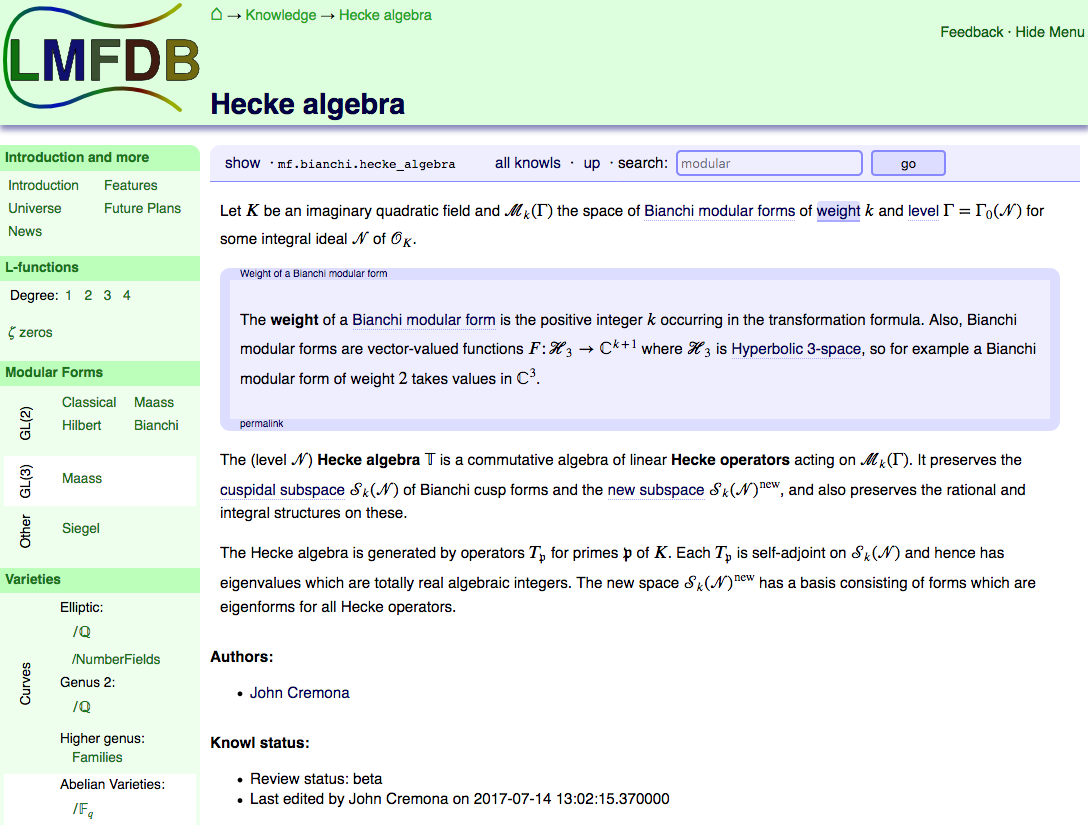
\includegraphics[width=14cm]{knowl}
  \caption{Knolws in the \LMFDB User Interface}\label{fig:knowl}
\end{figure}

\subsection{Alignments}\label{sec:integrating:alignments}

Finally we have to curate the \textbf{alignments} between the system dialects and the MitM ontology. 

To make the systems interoperable and translate objects and expressions, it is crucial to inform the system which symbols in the 
respective system API theories represent the same mathematical concepts. Then translation (as a first approximation) reduces to simply substituting symbols in an expression (see example below).\medskip

However, even when $A$ and $B$ deal with the ``same mathematical objects'', these may be constructed and represented differently, e.g., symbols can differ in name,
argument order/number, types, etc.
A major difficulty for system interoperability is correctly handling these subtle differences.
To formalize the details of this relation, \cite{MueGauKal:cacfms17} introduced \OMMT \textbf{alignments}.
Technically, these are pairs of \OMMT symbol identifiers decorated by a set of key-value pairs.
The alignments of $a$-symbols with the MitM ontology determine which $A$-objects correspond to MitM-objects.

The alignment of $a$-symbols to ontology symbols must be spelled out manually.
But this is usually straightforward and easy even for inexperienced users. For example, the following line aligns GAP's symbol \textsf{IsCyclic} (in the file \lstinline|lib/grp.gd|) with the corresponding symbol \textsf{cyclic} in the MitM ontology.
The key-value pairs are used to signify that this alignment is part of a group of alignments called ``VRE'' and can be used for translations in both directions.

\begin{lstlisting}
gap:/lib?grp?IsCyclic  mitm:/smglom/algebra?group?cylic
    direction="both" type="VRE"
\end{lstlisting}

Thus we can reduce the problem of interfacing $n$ systems to
\begin{inparaenum}[\em i\rm)]
\item curating the MitM ontology for the joint mathematical domain,
\item generating $n$ theory graphs for the system dialects,
\item maintaining $n$ collections of alignments with the MitM ontology.
\end{inparaenum}\medskip

For an example, consider again the dihedral group $D_4$ in \Sage (see Listings \ref{lst:sagedihedral:om} and \ref{lst:sagedihedral:xml}). We can align the relevant symbol 
\begin{lstlisting}
sage:?sage.groups.perm_gps.permgroup_named?DihedralGroup
\end{lstlisting}
with an abstract representation of dihedral groups in the MitM ontology (say, for instance \lstinline|mitm:?group?dihedralGroup|).
The \MMT system, when translating from \Sage to e.g. \GAP, then knows to replace the sage-specific symbol \lstinline|?DihedralGroup| by its system neutral equivalent in MitM, and the complex expression \lstinline+make_integer(4)+ by the plain OpenMath integer 4. To translate the resulting statement in MitM to \GAP, we only need to align \lstinline+mitm:?Groups?dihedralGroup+ with the constructor for dihedral groups in \GAP, namely \lstinline+gap:/grp?basic?DihedralGroupCons+. Translating to \GAP is then merely a matter of substituting this symbol in the OpenMath expression (\GAP already uses OpenMath integers for remote procedure calls via \SCSCP) to reconstruct the original \Sage object in \GAP. This yields the stepwise translation given in Figure \ref{fig:sagetogap}
\medskip

\begin{figure}\label{fig:sagetogap}

\begin{lstlisting}
sage:?sage.groups.perm_gps.permgroup_named?DihedralGroup
	mitm:?group?dihedralGroup 
	direction="both" type="VRE"
gap:/grp?basic?DihedralGroupCons							
	mitm:?group?dihedralGroup 
	direction="both" type="VRE"
\end{lstlisting}\medskip

\begin{tabular}{|lp{0.6\textwidth}|}\hline
\Sage & \lstinline|DihedralGroup(4)| \\
OpenMath (\Sage Dialect) & See Listing \ref{lst:sagedihedral:om} \\
OpenMath (MitM) & \lstinline|OMApplication(elem=OMSymbol(name='dihedralGroup', cd='group', cdbase='mitm'),arguments=[OMInteger(4)])| \\
OpenMath (\GAP Dialect) & \lstinline|OMApplication(elem=OMSymbol(name='DihedralGroupCons', cd='basic', cdbase='http://www.gap-system.org/grp'),arguments=[OMInteger(4)])| \\
	\GAP & \lstinline|DihedralGroupCons(4)|
\end{tabular}

\caption{Alignments and Stepwise Translation of Dihedral Group $D_4$ from \Sage to \GAP}
\end{figure}

Alignments form an independent part of the MitM interoperability infrastructure.
Incidentally, they obey a separate development schedule: the MitM ontology is developed by the community as a whole as the understanding of a mathematical domain changes.
The system dialects are released together with the systems according to their respective development cycle.
The alignments bridge between them and have to mediate these cycles.

These alignments are currently produced and curated using the approach, repository, and syntax described in~\cite{MueGauKal:cacfms17,MueRoYuRa:abtafs17}.
In the future, we will also consider automatically extracting alignments from the existing ad-hoc \Sage-to-$X$ translations.
These are (mainly) given as \Sage code annotations that relate \Sage operations and constructors with those of system $X$.

Figure~\ref{fig:cgtontology} shows some example alignments between symbols in the GAP content dictionary and the MitM ontology.




%%, but from some of the initial alignments and the \GAP API theories we will be able to infer more alignments automatically.
%%For example, the filter \texttt{GAP:IsGroup} is aligned with
%%\texttt{mitm:Group}, and the filter \texttt{GAP:IsPermGroup} is aligned with
%%\texttt{mitm:Subgroup SymmetricGroup [1..n]}.
%
%We formalized the theory of symmetric groups of a set in the MitM ontology.
%In \GAP, permutation groups are represented as subgroups (with finite support) of the symmetric group of $\mathbb{N}+$, and often one concretely has an isomorphism between the group one is interested in and a subgroup of $S_{\mathbb{N}+}$, for example via a group action.

%\texttt{SylowSubgroup}s are more difficult: They are special groups in their own right, namely groups whose size is a prime-power, but we also want them to be identified with a certain subgroup of the group we are working with.
%\ednote{MP: While I believe this to be an excellent additional example for \OMMT formalisation, this could be going too far for this paper}

%\ednote{MK@MK: still to write: the alignment-based priorization and suggestion mechanism. }


%%% Local Variables:
%%% mode: latex
%%% TeX-master: "report"
%%% End:

%  LocalWords:  DehKohKon:iop16 emph serialization sec:mitm deserializes subsubsection MueGauKal:cacfms17 MueRoYuRa:abtafs17 defemph defemph texttt texttt texttt texttt compactenum serializes lst:sagedihedral papertype ednote subtyping Cremona:LMFDB16,lmfdb:on knowls fig:knowl knowl knowl Kohlhase:ulsmf08 pdflatex flexiformal centering includegraphics Knolws inparaenum medskip MueGauKal:cacfms17,MueRoYuRa:abtafs17
%  LocalWords:  analyze itemize Deserialization serialized lstlisting pg_unreduce mathbb
%  LocalWords:  unpickle_global unreduce pg_DihedralGroup serializer py-openmath:on
%  LocalWords:  lstinline optimizations factorization serialize deserialized deserializer
%  LocalWords:  fig:cgtontology GroupHomset serializing analyzed py-scscp:on mitm:Group
%  LocalWords:  mitm:Subgroup SylowSubgroup newpart priorization summarize compactitem
%  LocalWords:  formalized
\newpage

\section[Databases]{Integrating Databases with MitM: LMFDB}\label{sec:databases}
The mathematical software systems to be integrated via the MitM approach have so far been computation-oriented, e.g., computer algebra systems.
Their API theories typically declare types and functions on these types (the latter including constants seen as nullary functions).
Even though database systems differ drastically from these in many respects, they are very similar at the MitM level: a mathematical database defines
\begin{compactitem}
 \item some types: each table's schema is essentially one type definition,
 \item many constants: each table entry is one constant of the corresponding type.
\end{compactitem}
Thus, we can reuse many of the same concepts.
In particular, the API theories must contain definitions of the database schemas. 

Apart from standard software engineering tasks, this leaves three conceptual problems we had to solve:
\begin{compactenum}[\bf P1]
\item Turn the database schemas and tables into \ommt theories and declarations. 
\item Lift data in \emph{physical} representation (as records of the
  underlying database) to \ommt object in \emph{semantic} representation.
\item Translate semantic queries to queries about physical representations so
  that they can be executed directly on the database without loading the entire theory into
  \mmt.
\end{compactenum}
We deal with \textbf{P1} in Section~\ref{sec:vt}, with \textbf{P2} in Section~\ref{sec:vt:codec}, and with \textbf{P3} in Section~\ref{sec:qmt}. 

In this paper, we focus on \lmfdb as an example, of which we give an overview in Section~\ref{sec:lmfdb}.
However, our methods are general enough to apply to many other mathematical databases such as OEIS, or findstat.

 \subsection{LMFDB Overview}\label{sec:lmfdb}
  \section{Example: The API and Structure of LMFDB}\label{sec:sota}

The ``L-Functions and Modular Forms Database'' (\lmfdb~\cite{lmfdb}) is a large database, storing among other mathematical objects several thousand L-Functions and curves along with their properties. 
Technically, it uses a MongoDB database with a Python web frontend. 
We use this as an example of a virtual theory. 
Before we go into this in more detail, we have a closer look at the structure and existing APIs to of \lmfdb.

\subsection{The Structure of LMFDB}\label{sec:sota:struct}

\lmfdb has several sub-databases, e.g., for elliptic curves or transitive groups. 
Within each of these, every object is stored as a single JSON record.
Figure~\ref{fig:lmfdbexample} shows an example: each property of this JSON object corresponds to a property of the underlying mathematical object. 
For example, the \identifier{degree} property -- here $1$ -- of the JSON objects corresponds to the degree of the underlying elliptic curve. 

\begin{figure}[ht]\centering
\begin{lstlisting}[language=json]
{
    "degree": 1,
    "x-coordinates_of_integral_points": "[5,16]",
    "isogeny_matrix": [[1,5,25],[5,1,5],[25,5,1]],
    "label": "11a1",
    "_id": "ObjectId('4f71d4304d47869291435e6e')",
    ...
}
\end{lstlisting}\vspace*{-1.5em}
  \caption[An elliptic curve from \lmfdb]{
    Part of an elliptic curve in \lmfdb (some fields omitted for brevity)
  }
  \label{fig:lmfdbexample}
\end{figure}

Other properties are more complex: the value of the \identifier{isogeny\_matrix} property is a list of lists representing a matrix. 
This disconnect between JSON encoding and mathematical meaning can become much more severe, e.g., the \identifier{x-coordinates\_of\_integral\_points} field is semantically a list of integers but (due to the sizes limits on integers) is encoded as a string.

\subsection{An API for \lmfdb Objects}\label{sec:sota:api}

\begin{wrapfigure}r{0.7\textwidth}\centering\vspace*{-2.5em}
  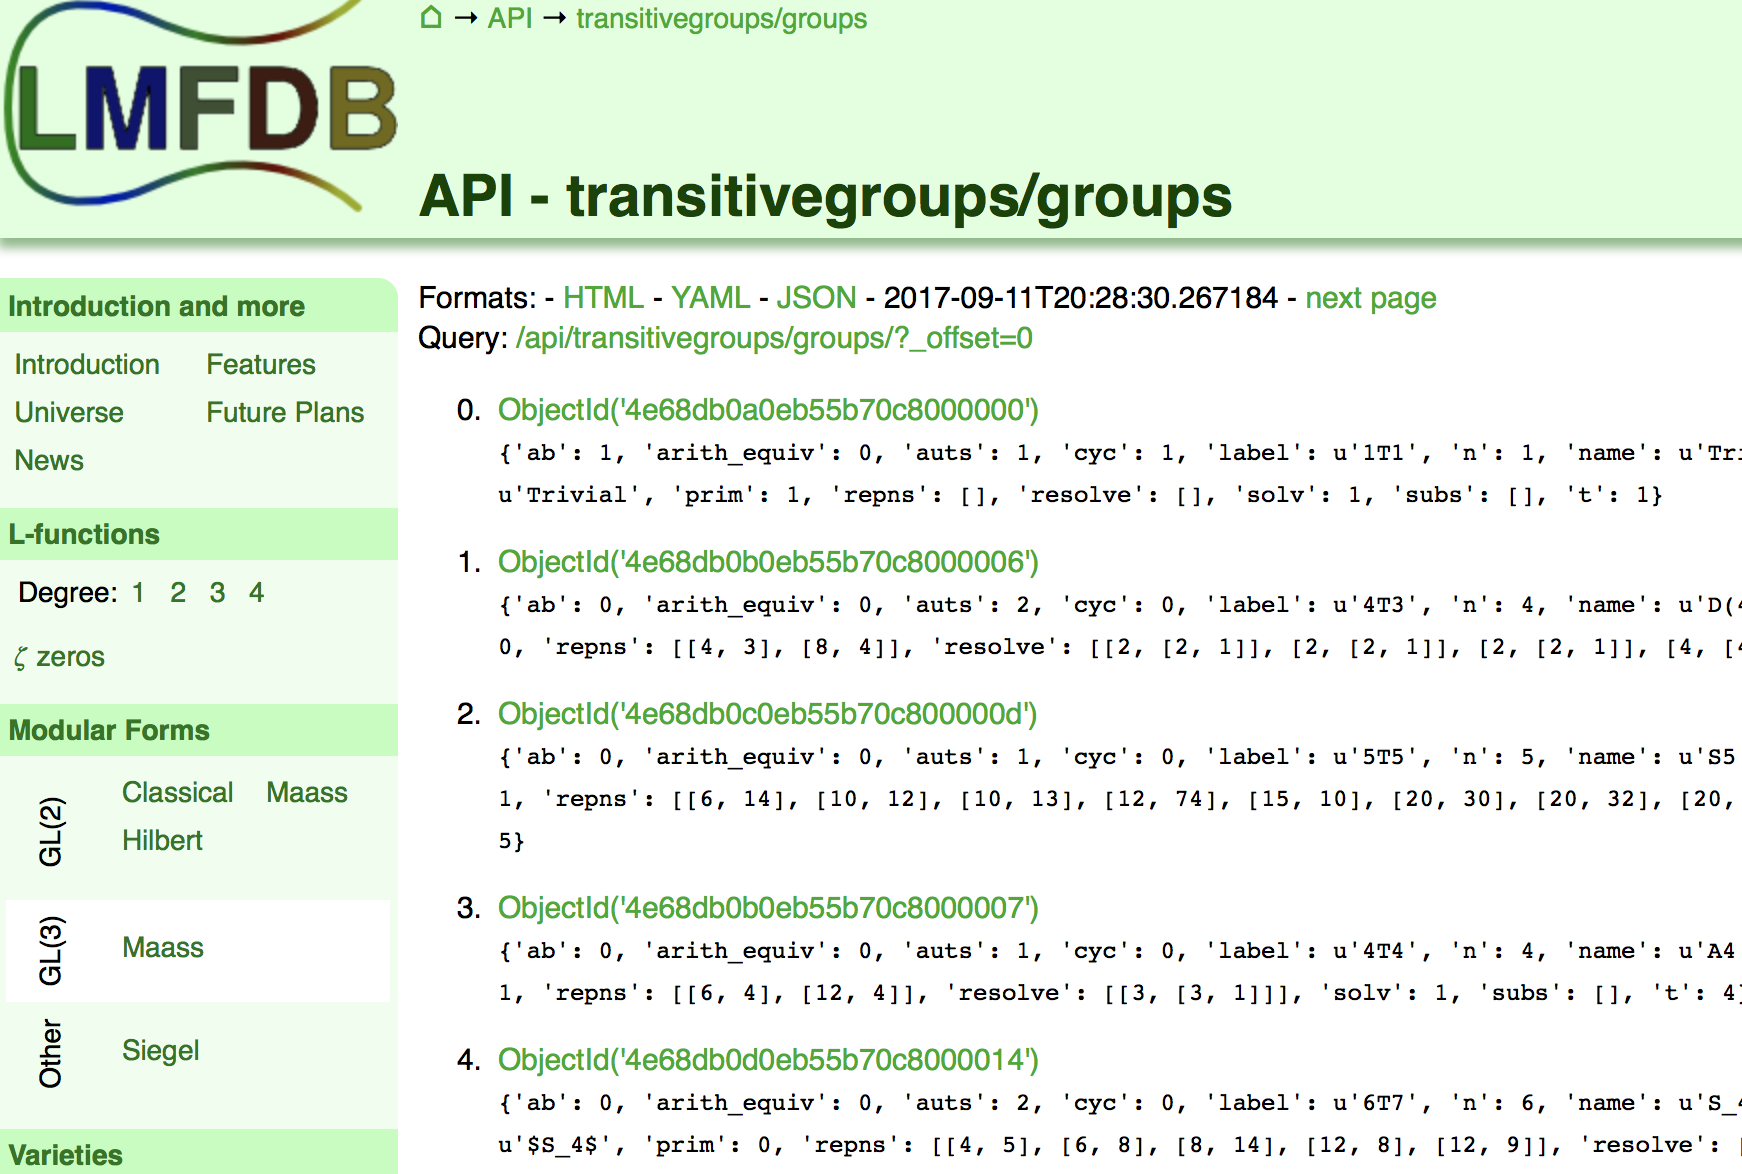
\includegraphics[width=0.7\textwidth]{APIScreenshot}
  \caption[The Web-Interface for the \lmfdb API. ]{
    The Web-Interface for the \lmfdb API. 
  }\vspace*{-1.5em}
  \label{fig:apiscreenshot}
\end{wrapfigure}
Querying is an important application for mathematical knowledge bases.
The \lmfdb API \cite{lmfdbapi} exposes a querying interface that can be used either by humans via the web or programmatically via JSON-based GET requests.
A screenshot of the former interface can be seen in Figure~\ref{fig:apiscreenshot}. 

Queries must name the sub-database to be queried and consist of a set of key-value pairs that correspond to an SQL \texttt{where} clause.
However, while \lmfdb offers a programmable API for accessing its contents, this API sits at the level of the underlying MongoDB, and not the level of mathematical objects. 
For example, to retrieve all Abelian objects in the subdatabase of transitive groups, we expect to use the key-value pair \identifier{commutative}$ = $ \identifier{true}. 
However, these values need to be encoded to be understood by MongoDB.
We need to realize that the database schema actually uses the key \identifier{ab} for commutativity, that it has boolean values, and that the schema encodes \inlinecode{true} as \inlinecode{1}. 
Thus, the actual query to send is \url{http://www.lmfdb.org/api/transitivegroups/groups/?ab=1}. 

In this example, all steps are relatively straightforward. 
But in general, e.g. when searching for all elliptic curves with a specific isogeny matrix, this not only requires good familiarity with the mathematical background but also with the system internals of the particular \lmfdb sub-database; a skill set commonly found in neither research programmers nor average mathematicians.   

Our diagnosis is that {\lmfdb} -- and most other mathematical knowledge databases -- suffer from two problems:
\begin{compactitem}
\item \emph{human/computer mismatch}: humans have problems interacting with \lmfdb because they must speak the system language instead of mathematical language
\item \emph{computer/computer mismatch}: mathematical computer systems cannot interoperate with \lmfdb because their system languages differ.
\end{compactitem}
Using the MitM approach we have presented in Section~\ref{sec:mmtmitm}, we can solve both problems at the same time by lifting the communication to the level of \ommt-encoded MitM objects, which both MitM-compatible software systems and humans can understand.
%%% Local Variables:
%%% mode: latex
%%% TeX-master: "paper"
%%% End:

%  LocalWords:  sec:sota lmfdb lmfdb lstlisting json ainvs iwp0 2adic_gens isogeny_matrix
%  LocalWords:  tamagawa_product 2adic_index anlist 4f71d4304d47869291435e6e vspace emph
%  LocalWords:  fig:lmfdbexample isogeny includegraphics textwidth fig:apiscreenshot
%  LocalWords:  centering summarize sec:mmtmitm ommt-encoded 4f71d4304d47869291435e6e
%  LocalWords:  serialization wrapfigure

 \subsection[Virtual Theories]{\lmfdb as a Set of Virtual Theories}\label{sec:vt}
  % !TEX root = ../thesis.tex
\section{Using Codecs To Implement \lmfdb Virtual Theories}\label{sec:vt}

From a system perspective, virtual theories behave just like concrete theories, but
without the assumption of loading all declarations from a file on disk at system startup.
Instead, virtual theories load declarations in a lazy fashion when they are
needed. Concrete theories are stored as XML files; i.e. we use the file system as a
backend for the \mmt system. As most of the knowledge sources we want to embed into \ommt
as virtual theories use data-bases as back-ends and provide low-level database APIs we
have extended the \mmt backends for this as well. Apart from standard software engineering
tasks, there were three conceptual problems to be solved in this extension/implementation:
\begin{compactenum}[\bf P1]
\item How to match the database tables into \ommt theories and declarations. 
\item How to lift data in \textbf{physical representation} -- i.e. as records of the
  underlying database to \ommt terms -- i.e. data in \textbf{semantic representation}.
\item And how to translate QML queries from semantic to physical representation -- i.e. so
  that they can be executed directly on the data base without loading bulk data into the
  \mmt process.
\end{compactenum}
We will discuss all three using the \lmfdb case discussed above as a running
example. \textbf{P1} can only be solved for each concrete application: Generally, we need
to represent \lmfdb as a set of \ommt theories.  As each sub-database in \lmfdb contains
records of similar structure, it makes sense to create a single virtual theory for each of
these sub-databases and use \ommt declarations for each of the objects. We address
\textbf{P2} next.

\subsection{Translating between Physical and Semantic Representations}\label{sec:vt:translation}

Consider, for example the \identifier{degree} field from the example above.  We have
already seen that this represents the degree of a curve and is an integer value, in this
case the integer $1$.  As \lmfdb uses MongoDB, which is based on JSON, integer values will
usually be represented as a JSON numbers, i.e. an \identifier{IEEE 754} $64$ bit floating
point number.  Here this is the floating point value $1.0$. But when the semantic
representations can exceed the have a maximum possible value $2^{53}-1$ of IEEE floats,
\lmfdb uses a different encoding, e.g. JSON strings that have no hard upper limit.

Let us call the set of objects in semantic representation the \textbf{semantic type}, and
the set of objects in the physical representation the \textbf{realized type}.  Semantic
types reside in the MiTM ontology, whereas realized types resides in the systems
themselves. Corresponding with intuition, the process of converting between the two
representations is called \textbf{coding}, specifically coding into a semantic
representation is called \textbf{encoding}, the reverse is called \textbf{decoding}. We
will call system components that do the necessary translation -- \underline{co}ding and
\underline{dec}oding -- \textbf{CoDec}s. 

As \ommt is a typed framework, we can directly use \ommt types from the MitM ontology for
the semantic types. Simple realized types are usually atomic database types whereas
complex realized types correspond to database tables or views; the details of this setup
are determined by the database schema. To arrive at a tight integration with the \ommt
functionality we will represent as much of this information in \ommt as possible.

Therefore we introduce a new \ommt theory \texttt{Codecs} in the foundational part of the
MitM ontology. See Figure~\ref{fig:vtarch} for details how this plays in the overall
information architecture and Figure~\ref{fig:codecs} for elementary content. This theory
introduces a type constructor \codectt, which given a semantic type constructs the type of
codecs for this type. For instance, the object \identifier{StandardPos} is (a CoDec) of
type $\codectt\;\mathbb{Z}^+$, i.e. a CoDec that parses database objects (for \lmfdb a
IEEE floats) into \ommt terms that can be typed as MitM positive integers and serializes
them back.

\begin{figure}[ht]\centering
  \begin{tikzpicture}\footnotesize
    \node[thy] (codecs) at (0,0) {
      \begin{tabularx}{.84\textwidth}{lll|X}
        \multicolumn{4}{l}{\textsf{Codecs}} \\\hline\hline   
        \identifier{codec}    & : & \multicolumn{1}{l}{$\typett\rightarrow\typett$} & \\\hline
        \identifier{StandardPos}    & : & $\codectt\; \mathbb{Z}^{+}$   & \multirow{3}{*}{\begin{minipage}{3.8in}
                                                                                      JSON number if small enough, \\
                                                                                      else JSON string of decimal expansion
                                                                                      \end{minipage}}\\
        \identifier{StandardNat}    & : & $\codectt\; \mathbb{N}$       & \\
        \identifier{StandardInt}    & : & $\codectt\; \mathbb{Z}$       & \\\hline
        \identifier{IntAsArray}     & : & $\codectt\; \mathbb{Z}$       & JSON List of Numbers\\
        \identifier{IntAsString}    & : & $\codectt\; \mathbb{Z}$       & JSON String of decimal expansion\\\hline
        \identifier{StandardBool}   & : & $\codectt\; \mathbb{B}$       & JSON Booleans \\
        \identifier{BoolAsInt}      & : & $\codectt\; \mathbb{B}$       & JSON Numbers $0$ or $1$ \\\hline
        \identifier{StandardString} & : & $\codectt\; \mathbb{S}$       & JSON Strings \\
      \end{tabularx}
    };
  \end{tikzpicture}
  \caption[List of Codecs]{
    An annotated subset of the Codecs theory containing a selection of codecs found in \mmt. 
    Here $\mathbb{N}$ represents natural numbers (including $0$), 
    $\mathbb{Z}$ integers, 
    $\mathbb{Z}^{+}$ positive integers, 
    $\mathbb{B}$ booleans and
    $\mathbb{S}$ (unicode character) strings. 
  }
  \label{fig:codecs}
\end{figure}
The \identifier{degree} we used as an example above would use the \identifier{StandardInt}
codec. Additionally the \textsf{CoDecs} theory associates with each codec a Scala class
that implements the translation between semantic and realized type.

But codecs for basic types (semantic and realized) is not sufficient for our application.
Consider for example the \identifier{isogeny\_matrix} field of an elliptic curve
representation.  The semantic representation of the value of this field is the matrix
\[M = \left(
    \begin{array}{ccc}
      1 & 5 & 25 \\
      5 & 1 & 5 \\
      25 & 5 & 1 \end{array} 
  \right)
\]
Matrices are characterized with three parameters, the type of object they contain
(integers in this case) along their row and column count ($3 \times 3$ in this case).  In
principle, one could construct a codec for each type of matrices by hand.  This would mean
generating one codec for $1 \times 1$ integer matrices, $1 \times 1$ real matrices,
$1 \times 2$ integer matrices, $1 \times 2$ real matrices, and so on.  For the
representation of codecs in \mmt, this would require generating one symbol and one Scala
function for each different kind of matrix.  This quickly becomes a mess.

Instead we use the fact that both Scala and \ommt allow higher-order functions: We can
define a \textbf{codec operator} that given a codec the parameter type $\tau$ and values
for the number $n$ of rows and $m$ of columns, generate a codec of $n\times m$ matrices of
$\tau$ objects. In the example above and the matrix $M$ is encoded as a list of $n$ lists
of $m$ integers ($\tau$):
% HACK HACK HACK overfull box\\\noindent
\inlinecode{[[1.0,5.0,25.0],[5.0,1.0,5.0],[25.0,5.0,1.0]]}

\begin{figure}[ht]\centering
  \begin{tikzpicture}\footnotesize
    \node[thy] (codecs) at (0,0) {
      \begin{tabularx}{\textwidth}{lll|X}
        \multicolumn{4}{l}{\textsf{Codecs (continued)}} \\\hline\hline   
        \identifier{StandardList}    & : & 
                 $\left\{T\right\} \codectt\; T \rightarrow \codectt\; \mathrm{List}(T)$ & 
                  JSON list, recursively coding each element of the list\\\hline
        \identifier{StandardVector}    & : & 
                  $\left\{T, n\right\} \codectt\; T \rightarrow \codectt\; \mathrm{Vector}(n, T)$ & 
                   JSON list of fixed length $n$\\\hline
        \identifier{StandardMatrix}    & : & 
                   $\left\{T, n, m\right\} \codectt\; T \rightarrow \codectt\; \mathrm{Matrix}(n, m, T)$ & 
                   JSON list of $n$ lists of length $m$\\
      \end{tabularx}
    };
  \end{tikzpicture}
  \caption[List of Codec Operators]{
    Second annotated subset of the codecs theory containing a selection of codec operators found in \mmt. 
    Compare with Figure~\ref{fig:codecs}. 
  }
  \label{fig:codecops}
\end{figure}
Like first-order codecs, codec operators in \mmt are again represented in two ways, as
declarations inside the \identifier{CoDecs} theory (see Figure~\ref{fig:codecops} for a
list) and as a corresponding Scala implementation -- a higher-order function from CoDecs
to CoDecs. This is mirrored in the types of operators in Figure~\ref{fig:codecs}: the
\textsf{StandardMatrix} operator is a function that takes four arguments: a type $T$, two
numbers $n$ and $m$, and a $\tau$-codec and yields a $\mathrm{Matrix}(n, m,
T)$-codec. Here we make use of the dependent function types of the MitM foundation:
arguments in curly brackets can be used in the result type; see~\cite{RabKoh:WSMSML13} for
details.

With these declarations in the \textsf{CoDecs} theory, we can represent a codec for
$3 \times 3$ integer matrices e.g. for the the isogeny matrix $M$ above by the \ommt term
$\plaintt{StandardMatrix}(3, 3, \plaintt{StandardInt})$\footnote{The observant reader will
  have noticed that the way codec operators have been declared, the codec in question
  actually corresponds to the term
  $\plaintt{StandardMatrix}(\mathbb{Z}, 3, 3, \plaintt{StandardInt})$.  This has an
  additional $\mathbb{Z}$ as the first argument.  However, the last argument is a codec
  for a specific semantic type and thus fully determines the first argument.  \mmt is
  capable of transparently inferring the first argument, thus it can be omitted for
  readability without needing any kind of special treatment implementation wise.  }.
Similarly the same codec operator can be used to for example generate a codec for
$2 \times 2$ boolean matrices, which corresponds to
$\plaintt{StandardMatrix}(2, 2, \plaintt{StandardBool})$.

\subsection{Schema Information in Virtual Theories}\label{sec:vt:schemas}

\begin{figure}[ht]\centering
    \begingroup
    \pgfdeclarelayer{background}
    \pgfdeclarelayer{foreground}
    \pgfsetlayers{background,foreground}
    
    \resizebox{\textwidth}{0.75\textwidth}{
      \begin{tikzpicture}[xscale=4,yscale=3]\footnotesize
        \begin{pgfonlayer}{foreground}
          \tikzstyle{human}    = [red,dashed,thick]
          \tikzstyle{withshadow}  = [draw,drop shadow={opacity=.5},fill=white]
          \tikzstyle{interface}   = [fill=blue!30]
          \tikzstyle{database}    = [cylinder,cylinder uses custom fill,
            cylinder body fill=yellow!50,cylinder end fill=yellow!50,
            shape border rotate=90,
            aspect=0.25,draw]
          
          % Ontology layer
          \node[thy] (numbers) at (0,1) {
            \begin{tabular}{lll}
              \multicolumn{3}{l}{\textsf{Numbers}}\\\hline\hline
              $\mathbb{Z}^{+}$        & : & \typett\\
              $\mathbb{Z}$            & : & \typett\\\hline
              \multicolumn{3}{l}{$\mathbb{Z}^{+} \subset \mathbb{Z}$}
            \end{tabular}
          };

          \node[thy] (matrices) at (1.5,1) {
            \begin{tabular}{lll}
              \multicolumn{3}{l}{\textsf{Matrices}}\\\hline\hline
              \plaintt{matrix} & : & $\typett \rightarrow \mathbb{Z}^{+}\rightarrow \mathbb{Z}^{+} \rightarrow \typett$
            \end{tabular}
          };

          \node[thy] (codecs) at (0.75,0) {
            \begin{tabular}{lll}
              \multicolumn{3}{l}{\textsf{Codecs}}\\\hline\hline
              \codectt                  & : & $\typett \rightarrow \typett$\\\hline
              \plaintt{standardInt}     & : & $\codectt\; \mathbb{Z}$\\
              \plaintt{standardMatrix}  & : & $\left\{T, n, m\right\} \codectt\; T \rightarrow \codectt\; \plaintt{matrix}(n, m, T)$\\
            \end{tabular}
          };

          \draw[include] (numbers) -- (matrices);
          \draw[include] (matrices) -- (codecs);
          
          \begin{pgfonlayer}{background}
            \node[draw=none,fill=green!30,rounded corners=1cm,fit=(numbers) (matrices) (codecs),inner sep=15pt] {};
          \end{pgfonlayer}
        
          % Model Layer
          \node[thy] (ec) at (2.25,-1.20) {
            \begin{tabular}{lll}
              \multicolumn{3}{l}{\textsf{Elliptic Curve}}\\\hline\hline
              \plaintt{ec}            & : & \typett\\\hline
              \plaintt{from\_record}  & : & $\plaintt{record} \rightarrow \plaintt{ec}$ \\\hline
              \plaintt{curveDegree}   & : & $\plaintt{ec} \rightarrow \mathbb{Z}$ \\
              \plaintt{isogenyMatrix} & : & $\plaintt{ec} \rightarrow \plaintt{matrix}(3, 3, \mathbb{Z})$ 
            \end{tabular}
          };

          \node[thy,interface] (ecschema) at (2.0,-2.5) {
            \begin{tabular}{lll}
              \multicolumn{3}{l}{\textsf{Elliptic Curve Schema}}\\\hline\hline
              $\plaintt{degree}$            & \uri{?implements}  & \plaintt{curveDegree} \\
                                            & \uri{?codec}       & \plaintt{StandardInt} \\\hline
              $\plaintt{isogeny\_matrix}$   & \uri{?implements}  & \plaintt{isogenyMatrix} \\
                                            & \uri{?codec}       & $\plaintt{StandardMatrix}(3, 3, \plaintt{StandardInt})$ 
            \end{tabular}
          };
          
          \begin{pgfonlayer}{background}
            \node[draw,cloud,fit=(ec),aspect=4,withshadow,inner sep=-4pt,purple!30] {};
          \end{pgfonlayer}

          % Database Layer
          \node[database] (mongodb) at (-.5,-2.5) {
            \textsf{\lmfdb Elliptic Curves}
          };

          \node[thy,interface] (dbtheory) at (0,-1.20) {
            \begin{tabular}{lllll}
              \multicolumn{5}{l}{\textsf{Elliptic Curve Database Theory}}\\\hline\hline
              \plaintt{11a1} & : & $\plaintt{ec}$ & $=$ & \dots\\
              \plaintt{11a2} & : & $\plaintt{ec}$ & $=$ & \dots\\
              \dots
            \end{tabular}
          };
          \draw[include] (matrices.south)+(.75,0) -- (ec.north);
          \draw[include] (ec) -- (dbtheory);
          
          \draw[human,->] (dbtheory) -- node[right]{\scriptsize {lazily loads from}} (mongodb);
          \draw[human,->] (ecschema) -- node[right]{\scriptsize {implements}} (ec);
          \draw[human,->] (ecschema) -- node[above]{\scriptsize {describes}} (mongodb);
        \end{pgfonlayer}
      \end{tikzpicture}
    }
    \endgroup
  \caption[Virtual Theory Architecture]{
    A sketch of the architecture for a virtual theory connecting to \lmfdb. 
    Solid edges represent imports. 
    Several declarations have been omitted for simplicity. 
  }
  \label{fig:vtarch}
\end{figure}

Codecs enable creation of individual values within \lmfdb and mathematical databases in general. 
This is not enough -- a mechanism to translate entire records as a whole is needed to implement a Virtual Theory. 

The architecture of a virtual theory for \lmfdb elliptic curves is illustrated in Figure~\ref{fig:vtarch}. 
It consists of four different parts, the foundational ontology theories (colored in green), mathematical model ontology (colored in red), database interface theories (colored in blue) and \lmfdb itself (colored in yellow). 
These aspects originate from the Math-In-The-Middle approach. 

The foundational ontology theories provide a system-independent basis for the remainder of the approach. 
In this example, they first define a type of integers $\mathbb{Z}$ and positive integers $\mathbb{Z}^{+}$ and then proceed to define a \identifier{matrix} type. 
This type takes three parameters, a type of elements in the matrix, and then a row and column count. 
Next, the codec \identifier{standardInt} and codec operator \identifier{standardMatrix} are defined as previously. 

Next, the \textit{Elliptic Curve} theory is described. 
It models an elliptic curve in a very simple fashion, by just declaring a type \identifier{ec}. 
Next, it defines a \identifier{from\_record} constructor that takes an \mmt record and returns an elliptic curve. 
Notice that these definitions are independent of the \lmfdb database. 

The theory then moves on to define the two important properties\footnote{In reality there
  are of course more than these two -- the others can be implemented analogously and are
  omitted here to better illustrate this example.} of elliptic curves.  These are
\textit{degree}, an integer, and the \textit{isogeny matrix}, a $3 \times 3$ matrix of
integers. They are modeled as functions that take an elliptic curve and return the
appropriate type.  Recall that the Math-In-The-Middle approach aims to model mathematical
knowledge ``in the middle'' independent of any particular system.  This is exactly the
case here -- the model of elliptic curves does not rely on \lmfdb, nor any other system,
so that we can integrate other knowledge sources about elliptic curves or to future
versions of the \lmfdb with changed struture.

\subsection{Knowledge Source Integration in MitM}

Given this infrastructure, let us see how we can integrate knowledge sources like the
\lmfdb in the Math-In-The-Middle approach. Instead of the API CDs presented in
Section~\ref{sec:mmtmitm}, we use an integrated approach that is based on \textbf{schema
  theory} that internalizes the \lmfdb schema and the \textbf{database theory}, a virtual
theory that represents the \lmfdb data.

The schema theory, as the name suggests, describes the schema of the \lmfdb elliptic curve
database.  This is the only place in the entire architecture of virtual theories which
relies on the structure of \lmfdb.  The schema theory contains declarations for each field
within an \lmfdb record.  The name of these declarations corresponds to the name of the
field inside the record.  Each declaration is annotated using \mmt meta-data with two
pieces of information, the property of an elliptic curve it implements and the codec that
is used to encode it inside \lmfdb.  For example, the \identifier{degree} field implements
the \identifier{curveDegree} property in the elliptic curve theory and uses the
\identifier{StandardInt} codec.

The other is the database theory. This is the truly virtual theory -- it is not stored on
disk, but generated dynamically.  As designed, it contains one declaration per record in
\lmfdb. It uses an \mmt \textbf{backend} -- an \mmt abstraction used to load declarations
into memory.  Given a URI, the backend is responsible for loading the underlying
definition.  For the elliptic curve theories these URIs are of the form
\uri{lmfdb:db/transitivegroups?groups?11A1}.\ednote{MK@TW: really transitive groups?}

The backend first retrieves the appropriate record from {\lmfdb} -- in the case of
\identifier{11A1} this corresponds to retrieving the JSON found in
Figure~\ref{fig:lmfdbexample}.  Next, the backend attempts to turn this JSON into an \mmt
record so that it can be passed to the \identifier{from\_record} constructor.

For this, it needs all declarations in the schema theory.  Each of these declarations
corresponds to a single field in the JSON, that can be turned into a field of the \mmt
record.  In the example provided here, we only consider two fields, \identifier{degree}
and \identifier{isogeny_matrix}.

For each of these two fields, the backend knows which field to create in the \mmt record
that it has to construct.  They are given by the \identifier{?implements} meta-datum, here
\identifier{curveDegree} and \identifier{isogenyMatrix}.  But this information is not
enough.  The JSON values of the fields can not be used as values inside an \mmt record,
they need to be assigned their correct semantics first.

This is where codecs and the \identifier{?codec} meta-datum come into play. 
The physical representation of the \identifier{degree} field is $1$, a JSON integer. 
The schema theory says that this is encoded using the \identifier{StandardInt} codec from above. 
To generate an \mmt value for the record, this codec can be used to decode it. 
In this case the decoded value is the integer $1$\footnote{
  In this document, the physical and semantic representation are rendered in the same fashion. 
  It is important to realize that they are not in fact the same. 
  The physical representation is a 64-bit floating point JSON Number $1$, whereas the semantic representation is the integer $1$. 
  Technically, the semantic representation is actually the \ommt integer literal $1$. 
  We skim over this detail here, as the \ommt literals are designed to precisely represent this value. 
}. 

The physical representation of \identifier{isogenyMatrix} is
\inlinecode{[[1.0,5.0,25.0],[5.0,1.0,5.0],[25.0,5.0,1.0]]}.  Here, the schema theory
contains a codec that is constructed using the \identifier{StandardMatrix} codec operator,
specifically \\$\plaintt{StandardMatrix}(3, 3,
\plaintt{StandardInt})$.  To apply this codec, the Backend has to first construct the
concrete codec, which can then used to decode the physical representation.  Since this is
a codec operator, first each entry of the matrix has to be decoded using
$\plaintt{StandardInt}$ -- turning the JSON number $1.0$ into the integer
$1$, the JSON Number $5.0$ into the number
$5$, etc.  Then these decoded values can be placed inside a matrix to arrive at the
semantic representation\footnote{Similar to the semantic representation above, the matrix
  $M$ is technically different from the \ommt representation.  We could again represent
  this using a matrix literal, but instead the implementation actually uses a constructor
  containing integer literals.  For simplicity, and as literals are designed to precisely
  represent mathematical objects, we omit this detail.  } 
\[M = \left( \begin{array}{ccc}
               1 & 5 & 25 \\
               5 & 1 & 5 \\
               25 & 5 & 1 
             \end{array}
           \right)
\]

This gives the backend all the information it needs to construct an \mmt record which can
then be turned into an elliptic curve using the \identifier{from\_record} constructor.
The \identifier{degree} field is assigned the value
$1$ and the \identifier{isogenyMatrix} is assigned the value of the matrix $M$.  Finally,
this \mmt term can be used to define a new constant inside the database theory.

%%% Local Variables:
%%% mode: latex
%%% TeX-master: "paper"
%%% End:

%  LocalWords:  sec:vt lmfdb ommt textit textit realized tikzpicture tabularx textwidth
%  LocalWords:  hline hline rightarrow codectt mathbb multirow fig:codecs isogeny mathrm
%  LocalWords:  characterized noindent formalized fig:codecops plaintt plaintt begingroup
%  LocalWords:  pgfdeclarelayer pgfsetlayers background,foreground resizebox xscale ec
%  LocalWords:  4,yscale pgfonlayer tikzstyle red,dashed,thick withshadow draw,drop oding
%  LocalWords:  cylinder,cylinder 50,cylinder 0.25,draw none,fill 30,rounded 1cm,fit
%  LocalWords:  thy,interface ecschema draw,cloud,fit 4,withshadow,inner 4pt,purple
%  LocalWords:  mongodb dbtheory endgroup fig:vtarch colored colored colored colored
%  LocalWords:  fig:lmfdbexample textbf centering RabKoh:WSMSML13 sec:mmtmitm
%  LocalWords:  internalizes

 \subsection{Ascribing Encodings in Schema Theories}\label{sec:vt:codec}
  % !TEX root = ../thesis.tex
\section{Accessing Virtual Theories}\label{sec:access}

We address \textbf{P2} next.
Intuitively, it is straightforward how to fill a virtual theory $V$: $V$ is represented by an initially empty concrete theory $V'$, and whenever an identifier $id$ of $V$ is requested, \mmt dynamically adds the corresponding declaration of $id$ to $V'$.
\mmt already abstracts from the physical realizations of persistent storage using the \emph{backend} interface: essentially a backend is any component that allows loading declarations.
Thus, we only have to implement a new backend that connects to \lmfdb, retrieves the JSON object with identifier $id$, and turns into an \ommt declaration.

However, this glosses over a major problem: the databases used for the physical storage of large datasets usually relatively simple data structure.
For example, a JSON database (as underlies \lmfdb) offers only limited-precision integers, boolean, strings, lists, and records as primitive objects and does not provide a type system.
Consequently, the objects stored in the database are very different from the sophisticated mathematical objects expected by the schema theory.
Therefore, databases like \lmfdb must encode this complex mathematical objects as simple database objects.

\subsection{Concrete Encodings of Mathematical Objects}\label{sec:vt:translation}

Consider, for example the \identifier{degree} field from Figure~\ref{fig:lmfdbexample} above. 
It's value is the integer $1$, representing the degree of this curve. 
However inside the database it is represented as the \identifier{IEEE 754} $64$-bit floating point number $1.0$. 
But when the semantic representations can exceed the have a maximum possible value $2^{53}-1$ of IEEE floats, \lmfdb needs to use a different encoding, e.g. JSON strings that have no hard upper limit.

Let us call the set of objects in semantic representation the \textbf{semantic type}, and the set of objects in the physical representation the \textbf{realized type}. 
Semantic types reside in the MiTM ontology, whereas realized types describe structures of the systems themselves -- here the tables in the \lmfdb. 
Corresponding with intuition, the process of converting between the two representations is called \textbf{coding}, specifically coding into a semantic representation is called \textbf{encoding}, the reverse is called \textbf{decoding}. 
We will call system components that do the necessary translation -- \underline{co}ding and \underline{dec}oding -- \textbf{CoDec}s. 

As \ommt is a typed framework, we can directly use \ommt types from the MitM ontology for the semantic types. 
Simple realized types are usually atomic database types whereas complex realized types correspond to database tables or views; the details of this setup are determined by the database schema. 
To arrive at a tight integration with the \ommt functionality we will represent as much of this information in \ommt as possible.

Therefore we introduce a new \ommt theory \texttt{Codecs} in the foundational part of the MitM ontology.  
See the green part of Figure~\ref{fig:vtarch} for details how this plays in the overall information architecture and Figure~\ref{fig:codecs} for elementary content. 
This theory introduces a type constructor \codectt, which given a semantic type constructs the type of CoDecs for this type. 
For instance, the object \identifier{StandardPos} is (a CoDec) of type $\codectt\;\mathbb{Z}^+$, i.e. a CoDec that parses database objects (for \lmfdb IEEE floats) into \ommt terms that can be typed as MitM positive integers and serializes them back.

\begin{figure}[ht]\centering
  \begin{tikzpicture}\footnotesize
    \node[thy] (codecs) at (0,0) {
      \begin{tabularx}{.84\textwidth}{lll|X}
        \multicolumn{4}{l}{\textsf{Codecs}} \\\hline\hline   
        \identifier{codec}    & : & \multicolumn{1}{l}{$\typett\rightarrow\typett$} & \\\hline
        \identifier{StandardPos}    & : & $\codectt\; \mathbb{Z}^{+}$   & \multirow{3}{*}{\begin{minipage}{3.8in}
                                                                                      JSON number if small enough, \\
                                                                                      else JSON string of decimal expansion
                                                                                      \end{minipage}}\\
        \identifier{StandardNat}    & : & $\codectt\; \mathbb{N}$       & \\
        \identifier{StandardInt}    & : & $\codectt\; \mathbb{Z}$       & \\\hline
        \identifier{IntAsArray}     & : & $\codectt\; \mathbb{Z}$       & JSON List of Numbers\\
        \identifier{IntAsString}    & : & $\codectt\; \mathbb{Z}$       & JSON String of decimal expansion\\\hline
        \identifier{StandardBool}   & : & $\codectt\; \mathbb{B}$       & JSON Booleans \\
        \identifier{BoolAsInt}      & : & $\codectt\; \mathbb{B}$       & JSON Numbers $0$ or $1$ \\\hline
        \identifier{StandardString} & : & $\codectt\; \mathbb{S}$       & JSON Strings \\
      \end{tabularx}
    };
  \end{tikzpicture}
  \caption[List of Codecs]{
    An annotated subset of the Codecs theory containing a selection of CoDecs found in \mmt. 
    Here $\mathbb{N}$ represents natural numbers (including $0$), 
    $\mathbb{Z}$ integers, 
    $\mathbb{Z}^{+}$ positive integers, 
    $\mathbb{B}$ booleans and
    $\mathbb{S}$ (unicode character) strings. 
  }
  \label{fig:codecs}
\end{figure}
The \identifier{degree} we used as an example above would use the \identifier{StandardInt} CoDec in the \lmfdb. 
Additionally the \textsf{CoDecs} theory associates with each CoDec a Scala class that implements the translation between semantic and realized type. The \mmt system we use is implemented in Scala and can thus execute this class as part of \lmfdb access. 

\begin{wrapfigure}r{2.7cm}\vspace*{-2em}
$M = \left(
    \begin{array}{ccc}
      1 & 5 & 25 \\
      5 & 1 & 5 \\
      25 & 5 & 1 \end{array} 
  \right)$\vspace*{-1em}
\end{wrapfigure}
But CoDecs for basic types (semantic and realized) are not sufficient for our application.
Consider again the \identifier{11a1} curve shown in Figure~\ref{fig:lmfdbexample}, specifically the \identifier{isogeny\_matrix} field. 
The semantic representation of the value of this field is the matrix on the right.

The semantic type of Matrices is characterized with three parameters, the type of object they contain (integers in this case) along their row and column count ($3 \times 3$ in this case). 
In principle, one could construct a CoDec for each type of matrices by hand. 
This would mean generating one CoDec for $1 \times 1$ integer matrices, $1 \times 1$ real matrices, $1 \times 2$ integer matrices, $1 \times 2$ real matrices, and so on. 
For the representation of CoDecs in \mmt, this would require generating one symbol and one Scala function for each different kind of matrix. 
This quickly becomes a mess.

Instead we use the fact that both Scala and \ommt allow higher-order functions: 
We can define a \textbf{CoDec operator} that -- given a CoDec, the parameter type $\tau$, and values for the number $n$ of rows and $m$ of columns --  generates a CoDec for $n\times m$ matrices of $\tau$ objects. 
In the example above and the matrix $M$ is encoded as a list of $n$ lists of $m$ integers ($\tau$):
\begin{lstlisting}[]
[[1.0,5.0,25.0],[5.0,1.0,5.0],[25.0,5.0,1.0]]
\end{lstlisting}

\begin{figure}[ht]\centering
  \begin{tikzpicture}\footnotesize
    \node[thy] (codecs) at (0,0) {
      \begin{tabularx}{\textwidth}{lll|X}
        \multicolumn{4}{l}{\textsf{Codecs (continued)}} \\\hline\hline   
        \identifier{StandardList}    & : & 
                 $\left\{T\right\} \codectt\; T \rightarrow \codectt\; \mathrm{List}(T)$ & 
                  JSON list, recursively coding each element of the list\\\hline
        \identifier{StandardVector}    & : & 
                  $\left\{T, n\right\} \codectt\; T \rightarrow \codectt\; \mathrm{Vector}(n, T)$ & 
                   JSON list of fixed length $n$\\\hline
        \identifier{StandardMatrix}    & : & 
                   $\left\{T, n, m\right\} \codectt\; T \rightarrow \codectt\; \mathrm{Matrix}(n, m, T)$ & 
                   JSON list of $n$ lists of length $m$\\
      \end{tabularx}
    };
  \end{tikzpicture}
  \caption[List of Codec Operators]{
    Second annotated subset of the CoDecs theory containing a selection of CoDec operators found in \mmt. 
    Compare with Figure~\ref{fig:codecs}. 
  }
  \label{fig:codecops}
\end{figure}
Like first-order CoDecs, CoDec operators in \mmt are again represented in two ways, as declarations inside the \identifier{CoDecs} theory (see Figure~\ref{fig:codecops} for a list, also compare again with Figure~\ref{fig:vtarch}) and as a corresponding Scala implementation -- a higher-order function from CoDecs to CoDecs. 
This is mirrored in the types of operators in Figure~\ref{fig:codecs}, the \textsf{StandardMatrix} operator is a function that takes four arguments: a type $T$, two
numbers $n$ and $m$, and a $\tau$-CoDec and yields a $\mathrm{Matrix}(n, m, T)$-CoDec. 
Here we make use of the dependent function types of the MitM foundation: arguments in curly brackets can be used in the result type; see~\cite{RabKoh:WSMSML13} for details.

With these declarations in the \textsf{CoDecs} theory, we can represent a CoDec for $3 \times 3$ integer matrices e.g. for the the isogeny matrix $M$ above by the \ommt term $\plaintt{StandardMatrix}(3, 3, \plaintt{StandardInt})$.
Similarly the same CoDec operator can be used to for example generate a CoDec for $2 \times 2$ boolean matrices, which corresponds to
$\plaintt{StandardMatrix}(2, 2, \plaintt{StandardBool})$. 

\subsection{Specifying Encodings in Schema Theories}

Given this infrastructure, let us see how we can integrate knowledge sources like the \lmfdb in the Math-In-The-Middle approach. 
The schema theory, as the name suggests, describes the schema of the \lmfdb elliptic curve database. 
This is the only place in the entire architecture of virtual theories which relies on the structure of \lmfdb. 
The schema theory contains declarations for each field within an \lmfdb record. 
The name of these declarations corresponds to the name of the field inside the record. 
Each declaration is annotated using \mmt meta-data with two pieces of information, the property of an elliptic curve it implements and the codec that is used to encode it inside \lmfdb. 
For example, the \identifier{degree} field implements the \identifier{curveDegree} property in the elliptic curve theory and uses the \identifier{StandardInt} codec.

The database theory is the only truly virtual theory -- it is not stored on disk, but generated dynamically. 
It can again be seen in Figure~\ref{fig:vtarch}. 
As designed, it contains one declaration per record in \lmfdb. 
It uses an \mmt \textbf{backend} -- an \mmt abstraction used to load declarations into memory. 
Given a URI, the backend is responsible for loading the underlying definition. 
For the elliptic curve theories these URIs are of the form \uri{lmfdb:db/elliptic_curves?curves?11A1}. 

The backend first retrieves the appropriate record from {\lmfdb} -- in the case of \identifier{11A1} this corresponds to retrieving the JSON found in Figure~\ref{fig:lmfdbexample}. 
Next, the backend attempts to turn this JSON into an \mmt record so that it can be passed to the \identifier{from\_record} constructor.

For this, it needs all declarations in the schema theory. 
Each of these declarations corresponds to a single field in the JSON, that can be turned into a field of the \mmt record. 
In the example provided here, we only consider two fields, \identifier{degree} and \identifier{isogeny_matrix}.

For each of these two fields, the backend knows which field to create in the \mmt record that it has to construct. 
They are given by the \identifier{?implements} meta-datum, here \identifier{curveDegree} and \identifier{isogenyMatrix}. 
But this information is not enough. 
The JSON values of the fields can not be used as values inside an \mmt record, they need to be assigned their correct semantics first.

This is where CoDecs and the \identifier{?codec} meta-datum come into play. 
The physical representation of the \identifier{degree} field is $1$, a JSON integer. 
The schema theory says that this is encoded using the \identifier{StandardInt} CoDecs from above. 
To generate an \mmt value for the record, this codec can be used to decode it. 
In this case the decoded value is the integer $1$. 
Notice how even though the physical and semantic representations are shown identically here, they are indeed different: The former is a 64-bit floating point JSON Number, the latter is a mathematical integer. 

The physical representation of \identifier{isogenyMatrix} is
% HACK HACK HACK -- TeX can't do proper line breaking
\\\noindent\inlinecode{[[1.0,5.0,25.0],[5.0,1.0,5.0],[25.0,5.0,1.0]]}. 
Here, the schema theory contains a CoDecs that is constructed using the \identifier{StandardMatrix} codec operator, specifically $\plaintt{StandardMatrix}(3, 3, \plaintt{StandardInt})$. 
To apply this CoDecs, the backend has to first construct the concrete CoDecs, which can then used to decode the physical representation. 
Since this is a CoDecs operator, first each entry of the matrix has to be decoded using $\plaintt{StandardInt}$ -- turning the JSON number $1.0$ into the integer $1$, the JSON Number $5.0$ into the number $5$, etc. 
Then these decoded values can be placed inside a matrix to arrive at the semantic representation of $M$. 

This gives the backend all the information it needs to construct an \mmt record which can then be turned into an elliptic curve using the \identifier{from\_record} constructor. 
The \identifier{degree} field is assigned the value $1$ and the \identifier{isogenyMatrix} is assigned the value of the matrix $M$. 
Finally, this \mmt term can be used to define a new constant inside the database theory.


%%% Local Variables:
%%% mode: latex
%%% TeX-master: "paper"
%%% End:

%  LocalWords:  sec:vt lmfdb ommt textit textit realized tikzpicture tabularx textwidth
%  LocalWords:  hline hline rightarrow codectt mathbb multirow fig:codecs isogeny mathrm
%  LocalWords:  characterized noindent formalized fig:codecops plaintt plaintt begingroup
%  LocalWords:  pgfdeclarelayer pgfsetlayers background,foreground resizebox xscale ec
%  LocalWords:  4,yscale pgfonlayer tikzstyle red,dashed,thick withshadow draw,drop oding
%  LocalWords:  cylinder,cylinder 50,cylinder 0.25,draw none,fill 30,rounded 1cm,fit
%  LocalWords:  thy,interface ecschema draw,cloud,fit 4,withshadow,inner 4pt,purple
%  LocalWords:  mongodb dbtheory endgroup fig:vtarch colored colored colored colored
%  LocalWords:  fig:lmfdbexample textbf centering RabKoh:WSMSML13 sec:mmtmitm
%  LocalWords:  internalizes

 \subsection{Translating Queries}\label{sec:qmt}
  % !TEX root = ../thesis.tex
Recall that \mmt has a general-purpose Query Language called QMT~\cite{Rabe:qlfml12}, which allows users to find knowledge subject to even complex conditions. 
We continue by briefly addressing \textbf{P3}: query translation; for a complete discussion we refer the interested reader to \cite{twiesing:msc17}. 

In practice, most queries involving virtual theories so far have a shape similar to the one that \lmfdb supports: 
Finding all objects within a single sub-database for which a specific field has a specific value. 
As an example, consider again the query of finding all Abelian transitive groups. 
QMT has an \mmt-powered surface syntax, which can be used to express this query as:
\begin{lstlisting}[language=qmt,basicstyle=\small\sf]
x in (related to ( literal `lmfdb:db/transitivegroups?group ) by (object declares)) 
  | holds x (x commutative x *=* true)
\end{lstlisting}

The example consists of two parts, first we find all objects declared in the \uri{lmfdb:db/transitivegroups?group} theory (line 1), and then we restrict this set of results to all those for which the \inlinecode{commutative} property is \inlinecode{true} (line 2). 
Notice that this the example shown here is the formal equivalent of the \lmfdb query shown in Section~\ref{sec:lmfdb}. 
The key difference is that this query does not require knowing the record structure of \lmfdb --
apart from knowing the proper sub-db, instead it only relies on knowing the mathematical
semantics (commutativity) of the query in question. 

Recall that to evaluate a query prior to the introduction of virtual theories, the \mmt system loaded the theory graph into main memory and then interleaved incremental flattening and query evaluation operations on the \mmt data structures until a result had been produced. 
But it is infeasible to first load all potentially relevant data into memory, and only then proceed with evaluation. 
This would require loading a copy of \lmfdb into main memory, something that virtual theories were designed to avoid. 

The low-level API of  \lmfdb and similar system provides a new approach for making queries towards virtual theories. 
First, the \mmt query is translated into a system-specific information-retrieval language --- in the case of \lmfdb\ this is currently a MongoDB-based syntax.
Next, this translated query is sent to the external API. 
Upon receiving the results, these are translated back into \ommt with the help of already existing functionality in the appropriate virtual theory backend.

This leaves just one problem unsolved --- translating queries into the system-specific API. 
However, it is insufficient to simply translate queries as a whole: 
One hand a general QMT query may or may not involve a virtual theory, on the other hand, it may also involve several (unrelated) virtual theories. 
This makes it necessary to filter out queries involving virtual theories, and assign them to a specific backend, and then translate only these parts. 

Achieving this automatically is a non-trivial problem. 
Queries are inductive in nature, and one could attempt to intercept each of the intermediate results. 
However, this would require a check on each intermediate result to first determine if it comes from a virtual theory or not, and then potentially switching the entire evaluation strategy, leading to a computationally expensive implementation. 

Instead of intercepting each result, we extended the Query Language to allow users to annotate sub-queries for evaluation with a specific virtual theory backend. 
This allows the system to immediately know which parts of a query have to be evaluated in \mmt memory, and which have to be translated and sent to an external system. 
This turns the example above into:
\begin{lstlisting}[language=qmt]
use "lmfdb" for {*
  x in (related to ( literal `lmfdb:db/transitivegroups?group ) 
    by (object declares)) | holds x (x commutative x *=* true)
*}
\end{lstlisting}
Here, we have simply wrapped the entire query with a \inlinecode{use lmfdb} statement, indicating the query should be evaluated using \lmfdb. 

The encoding of this specific query can be achieved using codecs.
The query corresponds to the URL \url{http://www.lmfdb.org/api/transitivegroups/groups/?ab=1}. 
Next, the \lmfdb API returns a set of JSON objects corresponding to all Abelian transitive groups. 
These can then be decoded into \ommt objects using the procedure described in Section~\ref{sec:vt:codec}, i.e. for each field we look up the corresponding codec and use it to deconstruct the field, eventually creating an \mmt record. 
Afterwards, these \ommt terms can then be passed to the user as a result to the query. 
%%% Local Variables:
%%% mode: latex
%%% TeX-master: "report"
%%% End:

%  LocalWords:  sec:qmt Rabe:qlfml12 textbf twiesing:msc17 lmfdb mmt-powered lstlisting
%  LocalWords:  qmt,basicstyle ommt qmt



%%% Local Variables:
%%% mode: latex
%%% TeX-master: "report"
%%% End:

%  LocalWords:  nullary compactitem compactenum ommt emph textbf textbf sec:qmt lmfdb qmt
%  LocalWords:  sec:lmfdb
\newpage
\section[Distributed Computation]{MitM-Based Distributed Computation}\label{sec:case}
\begin{figure}[ht]\centering\vspace*{-1em}
  \tikzinput{gap_singular_mitm_fig}
  \caption{MitM Interaction in Jane's Use Case}\label{fig:mitmpoc}\vspace*{-1em}
\end{figure}

Figure~\ref{fig:mitmpoc} shows the overall architecture with an MitM server as the central mediator.
All arrows represent the transfer of \OMMT objects via SCSCP.
Critically, the MitM server also maintains the alignments and uses them to convert between system dialects.

We have extended the \MMT system~\cite{Rabe:MAGMS13} with an SCSCP server/client so that it can receive/send objects from/to computation systems.
For the \GAP server, we built on pre-existing \SCSCP support.
To obtain an \SCSCP server for \Singular, which does not have native \SCSCP support, we wrapped \Singular in a python script that includes the \lstinline|pyscscp| library~\cite{py-scscp:on}.
In \Sage, we directly programmed the client interface to the MitM server. 

The resulting system forms the nucleus of the OpenDreamKit interoperability layer. It can already delegate computations between the three participating systems as long as the exchanged objects are covered by the MitM ontology, the alignments, and the formalizations of the system dialects.

\paragraph{Jane's Use Case} 
Initially, Jane has already built in \Sage the ring $R=\mathbb{Z}[X_1,X_2,X_3,X_4]$, the group $G=D_4$, the action $A$ of $G$ on $R$ that permutes the variables, and the polynomial $p = 3\cdot X_1 + 2\cdot X_2$.  She now calls
\begin{lstlisting}
  MitM.Singular(MitM.Gap.orbit(G, A, p)).Ideal().Groebner().sage()
\end{lstlisting}
which results in the following steps (the numbers on the edges of the
graph of Figure~\ref{fig:mitmpoc} indicate the order of communications when processing Jane's use case):
\begin{compactenum}
  \item Jane uses \Sage to call the MitM server with the command above, which includes both the computation to be performed and information about which system to use at which step.
  \item The MitM server translates \lstinline|MitM.Gap.orbit(G, A, p)| to the \GAP system dialect and sends it to \GAP.
  \item \GAP returns the orbit:
    \begin{displaymath}
      \begin{split}
        O = [3X_1 + 2X_2, 2X_3 + 3X_4, 3X_2 + 2X_3, 3X_3 + 2X_4,\\
        2X_2 + 3X_3, 3X_1 + 2X_4, 2X_1 + 3X_4, 2X_1 + 3X_2]\,.
      \end{split}
    \end{displaymath}
  \item The MitM server translates \lstinline|MitM.Singular(O).Ideal().Groebner()| to the \Singular system dialect and sends it to \Singular.
  \item \Singular returns the Gröbner base $B$.
  \item The MitM server translates $B$ to the \Sage system dialect and sends it to \Sage, where the result is shown to Jane.
    \begin{displaymath}
      B = [X_1 - X_4, X_2 - X_4, X_3 - X_4, 5X_4]\,.
    \end{displaymath}
  \end{compactenum}

\paragraph{Alternative Use Case}
Suppose Jon, one of Jane's colleagues, prefers working in \GAP, and he wants to
compute the Galois group of the rational polynomial $p = x^5 - 2$. He discovers
the \GAP package \texttt{radiroot}, which promises this functionality, but
unfortunately the package does not work for this polynomial and thus \GAP alone
cannot solve Jon's problem.

Jon hears from Jane that he should use \Sage, because she knows it can
compute Galois groups. So, from \GAP, he calls
\begin{lstlisting}
  G := MitM("Sage", "GaloisGroup",p)
\end{lstlisting}
which gives him the desired
Galois group as a \GAP permutation group. Having heard of Jane's
experiments, he can further run her orbit and Gröbner basis
calculation starting from this new group, without leaving his
favorite computing environment.
%\begin{lstinline}
%  G := MitM("Sage", "GaloisGroup",p)|

Finally, Jon, being a proficient \GAP user, also knows that he can now install a \defemph{method} in \GAP by calling 
\begin{lstlisting}
  InstallMethod(GaloisGroup, "for a polynomial", [IsUnivariatePolynomial], 
                p -> MitM("Sage", "GaloisGroup", p))
\end{lstlisting}
that will compute the Galois group of any rational polynomial transparently for him whenever he calls \lstinline|GaloisGroup| for a rational polynomial in \GAP. 
And thus (at the price of using multiple systems) a significant part of the 1800-line \lstinline|radiroot| package can be replaced by a few lines in GAP, taking advantage of the work of the \Sage community and participating in any future improvements of \Sage. 
In fact, Sage itself delegates to the PARI system -- another one of the OpenDreamKit systems -- for this computation.  So in the future \GAP might directly delegate to PARI instead, bypassing the need of iterated translations.

% $p =x^4-x^3-x^2+x+1$ over $\mathbb{Q}$ would have D_8 as galois group again...

%%% Local Variables:
%%% mode: latex
%%% TeX-master: "report"
%%% End:

%  LocalWords:  sec:case fig:mitmpoc IanJucKoh:sdm14,MathHub:on summarize sec:cgt pyscscp vspace lstlisting
%  LocalWords:  twiesing:msc17 centering tikzinput gap_singular_mitm_fig lstinline emph
%  LocalWords:  py-scscp:on oldpart mathbb cdot cdot Groebner Gröbner radiroot jist
%  LocalWords:  GaloisGroup galois
\newpage

\section{Conclusion}\label{sec:concl}
\section{Conclusion}\label{sec:concl}

We have shown how to extend the Math-in-the-Middle framework for integrating systems to mathematical data bases like the \lmfdb. 
The main idea is to embed knowledge sources as virtual theories, i.e. theories that are not -- theoretically or in practice -- limited in the number of declarations and allow dynamic loading and processing. 
For accessing real-world knowledge sources, we have developed the notion of codecs and integrated them into the MitM ontology framework. 
These codec's (and their MitM types) lift knowledge source access to the MitM level and thus enable object-level interoperability and allow humans (mathematicians) access using the concepts they are familiar with. 
Finally, we have shown a prototypical query translation facility that allows to delegate some of the processing to the underlying knowledge source and thus avoid thrashing of virtual theories. 

\paragraph{Related Work} Most other integration schemes employ a \textbf{homogenous approach}, where there is a master sytsem and all data is converted into that system. 
A paradigmatic example of this is the Wolfram Language and the Wolfram Alpha search engine~\cite{WolframAlpha:on}, which are based on the Mathematica kernel. 
This is very flexible for anyone owning a Matheamtica license and experienced in the Mathematica language and environment.

The MitM-based approach to interoperability of data sources and systems proposed in this paper is inherently a \textbf{heterogeneous approach}: systems and data sources are kept ``as is'', but their APIs are documented in a machine-actionable way that can be utilized for remote procedure calls, content format mediation, and service discovery. 
As a consequence, interaction between systems is very flexible.
For the data source integration via virtual theories presented in this paper this is important. 
For instance, we can just make an extension of \mmt or Sage which just act as a programmatic interface for e.g. \lmfdb. 

\paragraph{Future Work}
We have discussed the MitM+virtual theories methodology on the elliptic curves sub-base of the \lmfdb, which we have fully integrated. 
We are currently working on additional \lmfdb sub-bases. 
The main problem to be solved is to elicit the information for the respective schema theories from the \lmfdb community. 
Once that is accomplished, specifying them in the format discussed in this paper and writing the respective codecs is straightforward. 

Moreover, we are working on integrating the the Online Encyclopedia of Integer Sequences (OEIS~\cite{Sloane:OEIS,oeis}). 
Here we have a different problem: the OEIS database is essentially a flat ASCII file with different slots (for initial segments of the sequences, references, comments, and formulae); all minimally marked up ASCII art. 
In~\cite{LuzKoh:fsarfo16} we have already (heuristically) flexiformalized OEIS contents in \ommt; the next step will be to come up with codecs based on this basis and develop schema theories for OEIS.

\subsubsection*{Acknowledgements}
The authors gratefully acknowledge the fruitful discussions with other participants of
work package WP6, in particular John Cremona on the LMFDB and Dennis M\"uller on early
versions of the \ommt-based integration. We acknowledge financial support from the
OpenDreamKit Horizon 2020 European Research Infrastructures project (\#676541).

%%% Local Variables:
%%% mode: latex
%%% TeX-master: "paper"
%%% End:

%  LocalWords:  sec:concl subsubsection ommt lmfdb itemize Sloane:OEIS,oeis LuzKoh:fsarfo16 flexiformalized MitM-based textbf utilized


\printbibliography
\end{document}

%%% Local Variables:
%%% mode: latex
%%% TeX-master: t
%%% End:

%  LocalWords:  maketitle newpage tableofcontents newpage newcommand xspace ednote mathdb
%  LocalWords:  standardize dktheories concl printbibliography pn textit mmt mitm emph
%  LocalWords:  WPref dksbases prioritized taskref organized delivref dkstheories
%  LocalWords:  githubissuedescription
